\documentclass{stylefiles/capstone}
\usepackage[most]{tcolorbox}
\usepackage{tikz}
\usetikzlibrary{shapes.geometric, arrows.meta, positioning, fit, backgrounds}
% Define styles for flowchart elements
\tikzstyle{process} = [rectangle, minimum width=2cm, minimum height=0.8cm, text centered, draw=black, fill=blue!20, text width=3.2cm, font=\scriptsize]
\tikzstyle{processwide} = [rectangle, minimum width=3cm, minimum height=0.8cm, text centered, draw=black, fill=blue!20, text width=6cm, font=\scriptsize]
\tikzstyle{decision} = [diamond, minimum width=2cm, minimum height=0.8cm, text centered, draw=black, fill=green!20, aspect=2, font=\scriptsize, text width=2cm]
\tikzstyle{arrow} = [thick,->,>=Stealth]
\tikzstyle{subgraph} = [rectangle, draw=black, dashed, inner sep=8pt]
\begin{document}

\title{Designing an Adaptive AI System for Personalized Learning Pathways Using Instructor-Guided Content}

%year
\capstoneyear{2026}
% options are Seminar, Project 1, Project 2
\capstonedocument{Project 2}
% options are Fall, Spring
\capstonesemester{Spring}

% Author info
\author{Moudjahid Nouroudini Moussa}
\affiliation{%
  \institution{Computer Science, NYUAD}
}
\email{mm12515@nyu.edu}

% Advisors
\advisors{Hanan Salam, Djellel Difallah}

\renewcommand{\shortauthors}{Moudjahid}

\begin{abstract}
Most AI-powered learning platforms offer static instruction sequences that ignore learner diversity. This capstone report covers two semesters of work on SynapsEd, a platform that generates and adapts personalized learning pathways using instructor-curated content. During the first semester, we built the core AI engine combining retrieval-augmented generation (RAG) and deep knowledge tracing (DKT), grounded all recommendations in instructor-approved materials, and validated design priorities through expert consultation with 8 educational specialists and 6 students. During the second semester, we extended the system with three new features grounded in cognitive science research: (1) a voice-based learning mode in which students speak to the AI tutor and receive spoken responses, operationalizing the modality principle from multimedia learning theory~\cite{mayer2021instructional,moreno2007interactive}; (2) a drawing-based visual explanation mode in which the AI generates Excalidraw diagrams for abstract or spatial concepts, triggered by student profile and concept type, following generative learning evidence~\cite{fiorella2016generative,rau2017visual}; and (3) a mastery-gated quiz system in which students complete in-chat assessments before formal quiz sections unlock, implementing Bloom's mastery learning model at scale~\cite{bloom1984sigma}. The second semester also produced two research outputs currently in preparation: a benchmark paper (SocraticRAG) evaluating whether LLMs can generate Socratic tutoring responses that stay faithful to retrieved course materials, targeting EMNLP 2026, and a longitudinal study evaluating SynapsEd with real students and instructors over the summer, targeting CHI 2027. This work contributes a model for bridging automated personalization with human-centered pedagogy in higher education.
\end{abstract}

\keywords{personalized learning, AI in education, retrieval-augmented generation, knowledge tracing, human-AI interaction, learning pathways}

\maketitle

\section{Introduction}

The popularization of generative AI has introduced exciting possibilities in education, particularly around adaptive and personalized learning. Yet transitioning to higher education represents a critical juncture where students encounter unprecedented academic demands while navigating diverse educational backgrounds. Many students enter university courses with varying levels of prerequisite knowledge, different learning preferences, and distinct goals that shape how they engage with material. Despite this diversity, most existing learning platforms apply one-size-fits-all models or linear content sequences that fail to account for individual learner variation. This mismatch between what learners know and what content they receive often results in disengagement, cognitive overload, or inadequate challenge~\cite{ausubel1978educational}.

Building on these challenges, numerous AI tutoring systems and adaptive learning platforms have emerged to help students manage coursework and receive personalized feedback. Commercial tools like YouLearn AI offer adaptive quizzes and chat support, Khan Academy and Duolingo leverage gamification and learner dashboards, and ChatGPT Study Mode provides on-demand tutoring through conversational AI. Google's NotebookLM enables AI-driven summaries from user-uploaded documents. These platforms represent significant advances in making learning more accessible and engaging. However, they are primarily designed as direct-to-student tools rather than classroom systems that support collaboration between instructors and learners. When instructors cannot curate the content foundation, review AI-generated recommendations, or access insights about class-level learning patterns, it becomes challenging to integrate these tools into structured curricula. Students benefit from personalized interactions, but instructors lack visibility into whether recommendations align with course objectives or pedagogical standards. This gap between individual learning support and classroom integration leaves educators seeking ways to harness AI's adaptive capabilities while maintaining their role as curriculum designers and pedagogical decision-makers~\cite{Herrmann-Werner2024,chaudhry2022transparencyindexframeworkai,mollick2023using}.

Given these considerations, there is an opportunity to design platforms that bridge individual personalization with classroom workflows. This capstone introduces SynapsEd, an adaptive system that creates personalized learning pathways while supporting collaboration between instructors and students. The platform addresses three core challenges: enabling instructors to maintain curriculum authority while benefiting from AI-driven adaptation, ensuring transparency so both instructors and students understand system reasoning, and dynamically adjusting to individual needs while preserving pedagogical integrity.

SynapsEd operates through a collaborative workflow where instructors upload course materials (syllabi, lecture slides, documents) that are processed into a semantically searchable knowledge base. Student survey responses capturing learning goals, prior knowledge, and preferences are combined with this content repository to generate personalized pathways. Each pathway consists of sequential learning nodes representing focused objectives with recommended resources, prerequisite relationships, and assessment opportunities. Instructors review and approve every pathway before deployment, ensuring alignment with course standards. As students progress, an intelligent tutoring agent uses retrieval-augmented generation to ground all responses in instructor-provided materials, maintaining content fidelity while adapting to student performance through knowledge tracing techniques~\cite{10933562}.

The system prioritizes transparency at every stage. Students understand why pathways are structured as they are, see source attributions for all tutoring responses, and receive explanations for adaptive recommendations. Instructors access aggregate analytics showing class-level patterns, common challenges, and content areas requiring additional support. This bidirectional information flow ensures that personalization remains anchored in approved curriculum while instructor decisions are informed by empirical evidence of student learning.

During the first semester, we built the core AI engine and validated the design through expert consultation with 8 educational specialists and 6 students. This report covers the full two-semester arc of that work. Our goal throughout has been to understand how adaptive learning systems can genuinely bridge individual student needs and classroom workflows, rather than serving students and instructors in isolation.

\section{Related Work}
\label{sec:related}

This project builds on research at the intersection of artificial intelligence, educational psychology, and human-computer interaction. We organize related work into five areas: existing commercial and academic platforms, the technical foundations enabling content retrieval and generation, pedagogical and ethical considerations for AI in education, research on adaptive learning systems, and multimodal and generative learning approaches that inform our Semester 2 feature design.

\subsection{Existing Platforms and the Classroom Integration Gap}

Academic work on AI-driven personalization demonstrates that these approaches can meaningfully improve learning outcomes, with personalized pathways showing a 25\% improvement in grades in higher education~\cite{NaseerFawad2024Idlt} and systems combining knowledge tracing with RAG achieving measurable gains in student engagement~\cite{Li}. But as described in the Introduction, most existing platforms, commercial and academic alike, are built around the student experience. Instructors cannot curate the content foundation, verify that recommendations align with course objectives, or see aggregate learning patterns across the class. SynapsEd is designed to occupy that middle ground.

\subsection{Retrieval-Augmented Generation}

Retrieval-Augmented Generation (RAG) represents a foundational technique for grounding AI responses in verified source materials. Lewis et al.~\cite{lewis2021rag} introduced this approach for knowledge-intensive NLP tasks, combining dense vector search with generative models to ensure responses are traceable to relevant documents rather than relying solely on model parameters. This architecture addresses the hallucination problem inherent in large language models by anchoring generation in retrieved evidence.

Recent advances have extended RAG capabilities to multimodal content processing. Vision Language Models (VLMs) such as those employed in ColPali enable systems to process not only text but also visual elements embedded in educational materials like diagrams, charts, and annotated slides ~\cite{faysse2025colpaliefficientdocumentretrieval}. This multimodal approach is particularly important in higher education where instructors communicate concepts through diverse formats. For SynapsEd, we leverage Mistral OCR to extract text from visual content in slide presentations and documents, ensuring that pedagogically significant visual materials become queryable within the semantic search system.

The effectiveness of RAG depends critically on chunking strategies that preserve semantic coherence. Rather than splitting documents at arbitrary token boundaries, semantic-aware chunking respects logical divisions such as section headers, paragraphs, and code blocks. This ensures that retrieved passages contain contextually complete information rather than fragmented snippets~\cite{lewis2021rag}. SynapsEd implements multi-layered markdown chunking that maintains these semantic boundaries while enabling fine-grained retrieval aligned with specific student queries.

\subsection{Pedagogical and Ethical Considerations}

While RAG provides technical infrastructure for grounded responses, its application in educational contexts raises important pedagogical and ethical considerations. Herrmann-Werner et al.~\cite{Herrmann-Werner2024} evaluated large language models on real-world exam questions, demonstrating that LLMs frequently underperform on foundational cognitive tasks when not grounded in expert-reviewed content. Their findings caution against over-reliance on LLMs for educational applications without mechanisms to verify accuracy and pedagogical appropriateness. SynapsEd directly addresses this concern by restricting all content retrieval to instructor-uploaded materials, ensuring that students never receive information that has not been vetted by course instructors.

Beyond accuracy, transparency represents a critical requirement for AI systems in education. Chaudhry et al.~\cite{chaudhry2022transparencyindexframeworkai} developed a comprehensive framework for evaluating transparency in educational AI, arguing that explainability benefits multiple stakeholders: students need to understand why content is recommended, instructors need visibility into system decision-making to maintain oversight, and system designers need feedback mechanisms to identify failures. Their framework emphasizes that transparency must be actionable, explanations should enable users to verify correctness, contest decisions, and provide meaningful feedback. SynapsEd operationalizes these principles through explicit source attribution for all tutoring responses, visual pathway representations showing prerequisite relationships and cognitive progression, and instructor-facing analytics that surface system reasoning.

Educational AI systems must also respect foundational learning principles established through decades of cognitive science research. Ausubel's theory of meaningful learning~\cite{ausubel1978educational} emphasizes that learners bring different levels of prior knowledge, which fundamentally affects how they absorb new information. Content that assumes too much background leads to confusion and disengagement, while content that fails to challenge sufficiently results in boredom. SynapsEd addresses this through diagnostic surveys that assess prerequisite knowledge and learning goals, enabling pathway generation to align content sequencing with individual starting points. Additionally, the system incorporates Bloom's taxonomy to ensure cognitive progression, starting with foundational knowledge before advancing to application, analysis, and synthesis.

\subsection{Adaptive Learning Systems Research}

Research in AI-driven adaptive learning has produced promising results across various educational contexts. TutorLLM combines knowledge tracing with RAG for content recommendations, demonstrating a 10\% increase in student satisfaction and 5\% improvement in quiz scores through adaptive sequencing~\cite{Li}. Vorobyeva et al.~\cite{Vorobyeva2025} and Barrera et al.~\cite{barrera2024personalized}, examining AI personalization in higher education, consistently find that the most effective implementations balance algorithmic efficiency with human judgment, where AI surfaces patterns and generates recommendations while instructors retain final pedagogical authority~\cite{zhang2024questioncentricmultiexpertscontrastivelearning}. Classroom adoption ultimately requires more than technical performance: instructors need mechanisms to review AI-generated content, students benefit from understanding why recommendations are made, and both need assurance that personalization aligns with course objectives.

A consistent finding across this literature is that deploying a capable LLM is not the same as having a capable tutor. Liu et al.~\cite{liu2024socraticlm} build a dataset of 35,000 Socratic-style dialogues and fine-tune models across five pedagogical dimensions, finding that ``current LLM-based application in personalized teaching predominantly follows a Question-Answering paradigm, where students are passively provided with answers and explanations.'' GPT-4, even when explicitly instructed to guide rather than tell, gives the answer directly. MathTutorBench~\cite{macina2025mathtutorbench}, the most comprehensive tutoring benchmark to date, confirms this from a different angle: ``subject expertise does not immediately translate to good teaching,'' and models that perform well on factual tasks fail on Socratic scaffolding, especially in longer conversations. Bonino et al.~\cite{bonino2024euler} fine-tune LLMs for Socratic interactions specifically and still find consistent failures in the most basic criterion: withholding the answer.

These findings directly shaped two decisions in SynapsEd. First, the tutoring agent's system prompt explicitly prohibits direct answers rather than relying on general instruction-following. Second, the parallel SocraticRAG benchmark project exists because even with explicit enforcement, we do not yet have a way to measure whether the agent's Socratic responses are faithful to the retrieved course materials, which is the gap that motivates the EMNLP paper.

\subsection{Multimodal and Generative Learning}

A growing body of research in educational psychology establishes that how information is delivered matters as much as what is delivered. Mayer~\cite{mayer2021instructional} and Moreno and Mayer~\cite{moreno2007interactive} show that splitting verbal and visual content across separate perceptual channels prevents cognitive overload and enables interactive dialogue. Fiorella and Mayer~\cite{fiorella2016generative} establish drawing as a research-validated generative learning strategy, with spatial and abstract material benefiting most. Rau~\cite{rau2017visual} reviews conditions under which visual representations enhance STEM learning, finding them especially effective for students with low prior knowledge. These four bodies of work motivate the two new modality features described in Section~\ref{sec:s2features}: voice-based interaction and AI-generated visual explanations.

\section{Summary of Work Across Both Semesters}

The first semester produced SynapsEd's complete foundational AI engine: a data ingestion pipeline that processes instructor-uploaded materials through OCR and semantic chunking, a survey generation engine that creates course-specific diagnostic questionnaires, a pathway generation module that builds personalized learning sequences pending instructor review, and an intelligent tutoring agent grounded in class materials using RAG and the Socratic method. Expert consultation with 8 educational specialists and 6 students validated the design. The second semester extended the system with three new features grounded in cognitive science research: voice-based interaction, AI-generated visual explanations using Excalidraw, and mastery-gated quizzes built on top of the existing DKT component. It also produced two research outputs in preparation: SocraticRAG, an NLP benchmark for retrieval-faithful Socratic tutoring evaluation targeting EMNLP 2026, and a longitudinal study evaluating SynapsEd with real students and instructors targeting CHI 2027.

\section{Methodology}
\label{sec:methodology}

\subsection{System Overview}

The system serves two primary user groups (instructors and students) each interacting with distinct but interconnected workflows designed to maintain pedagogical control while enabling individualized learning experiences. Figure~\ref{fig:overall_system} illustrates the complete system architecture and how the instructor and student workflows interconnect.

\begin{figure}[h]
\centering
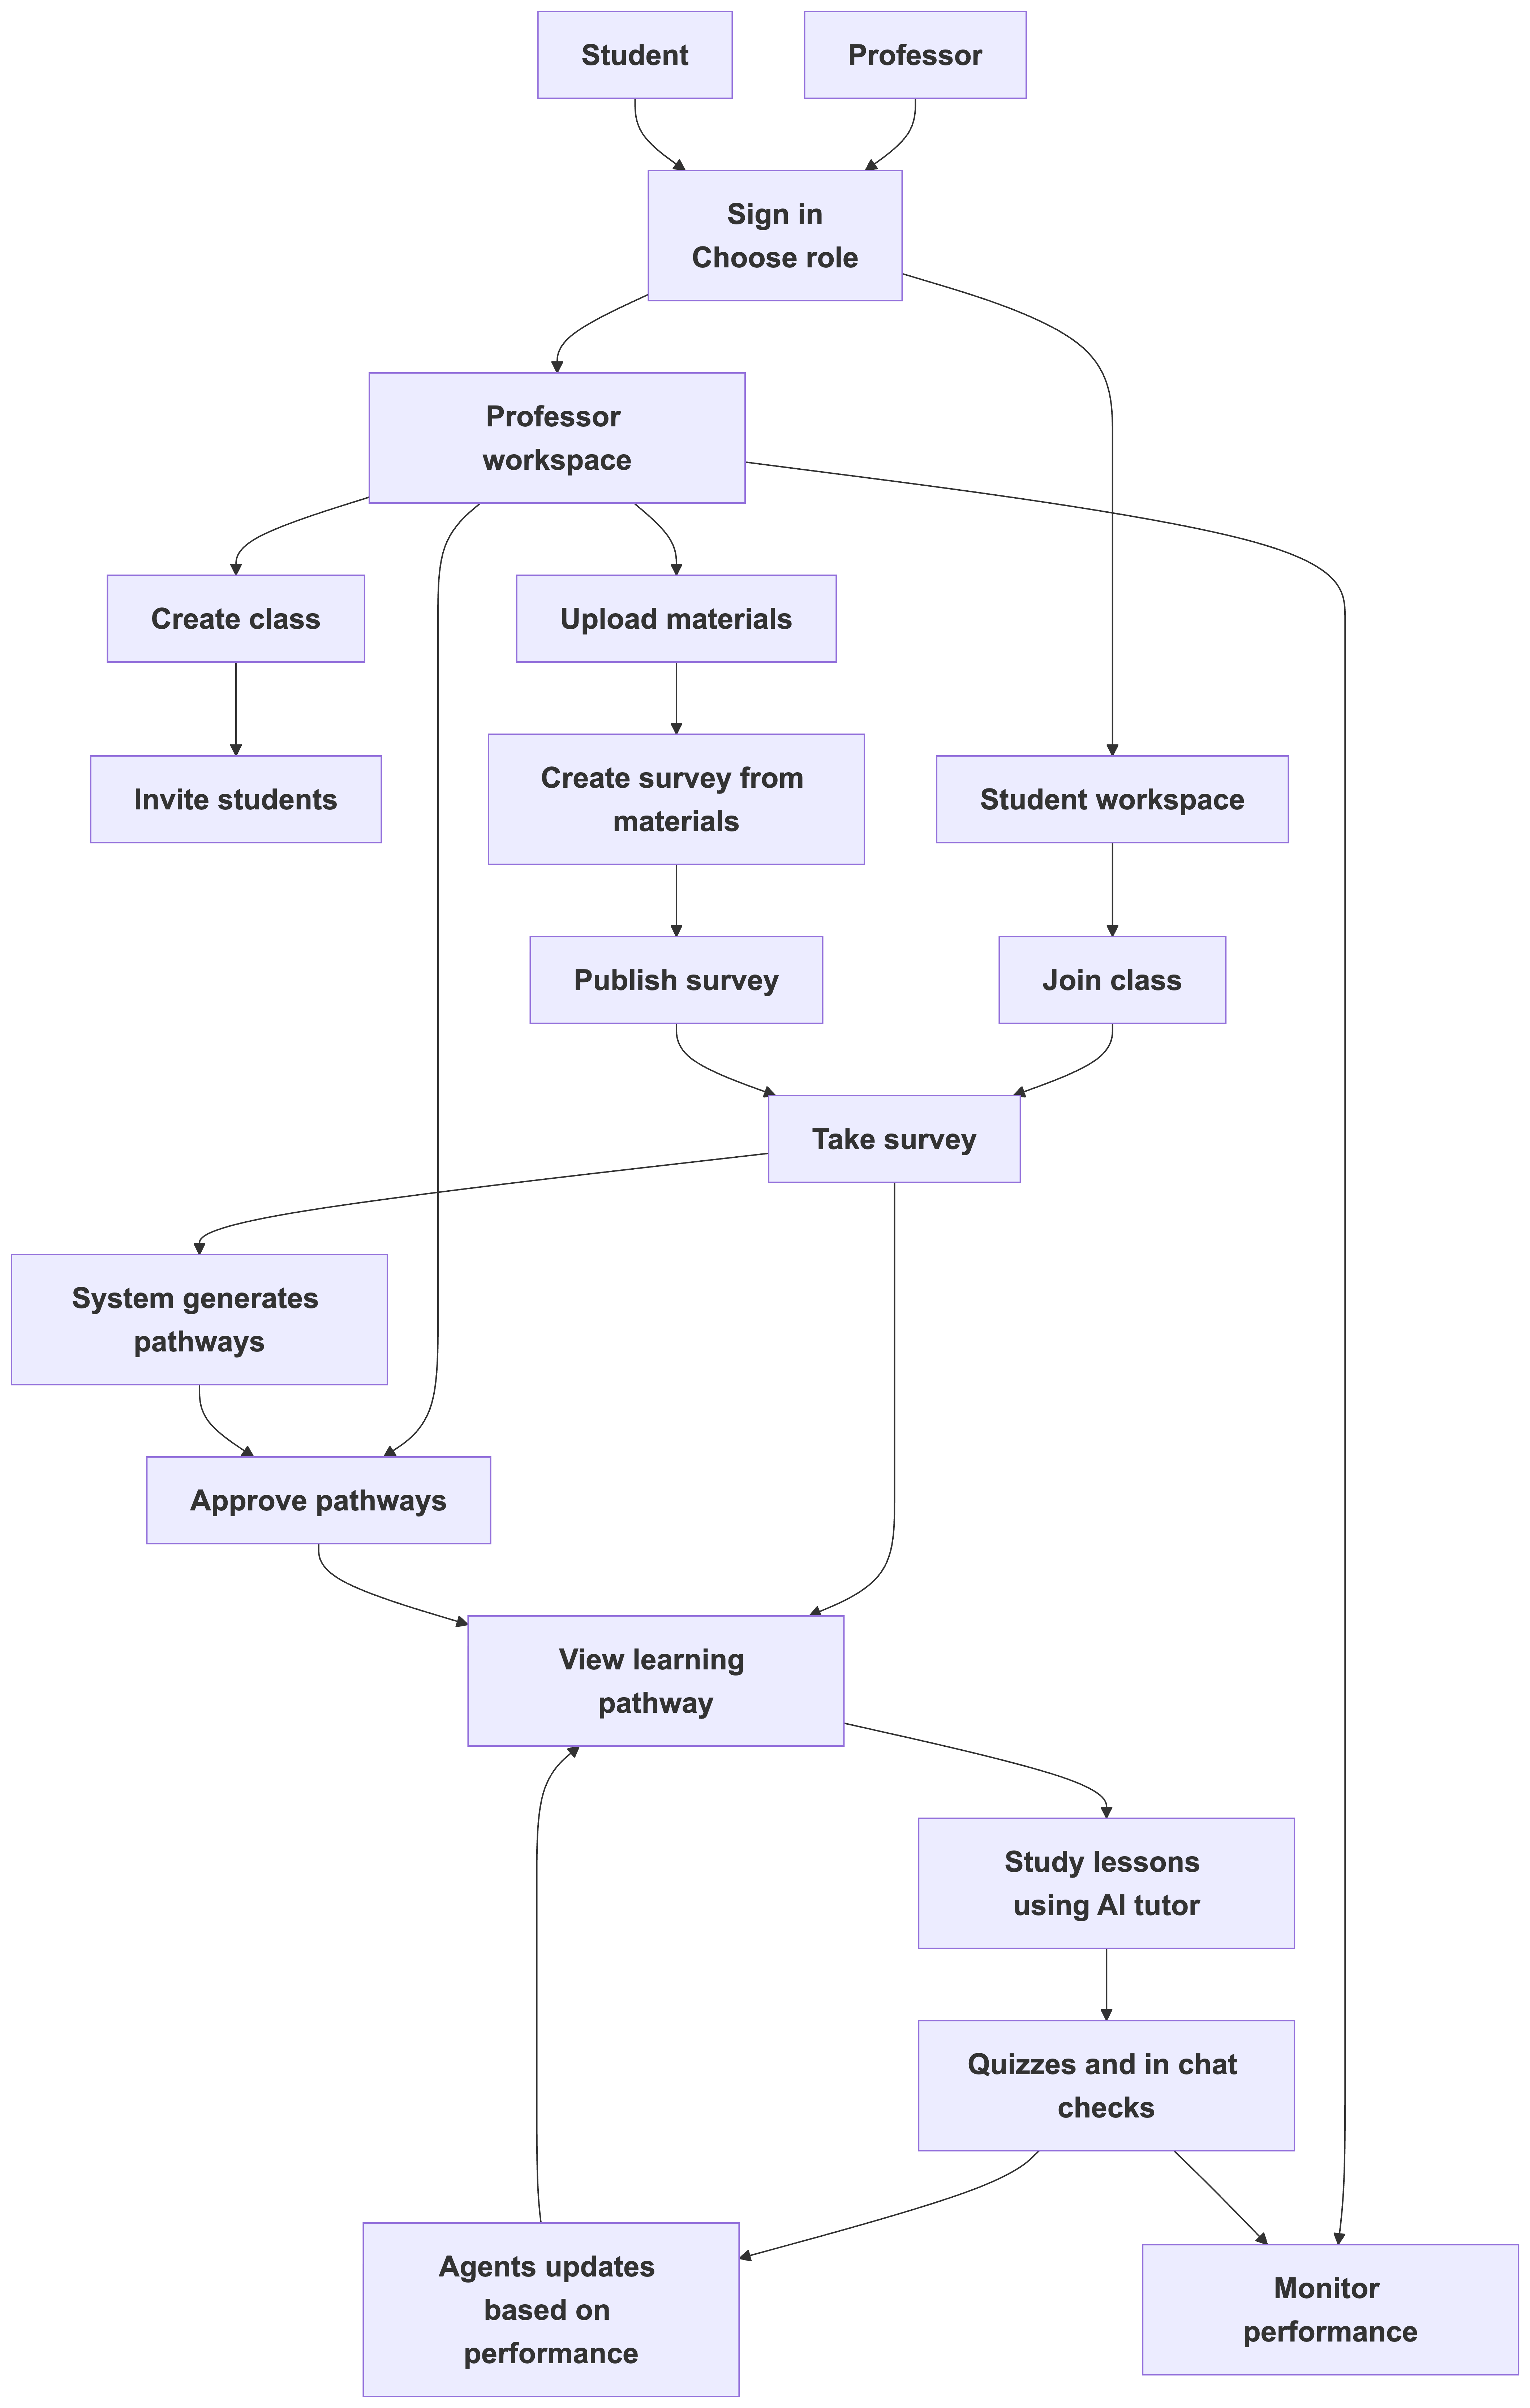
\includegraphics[width=1\columnwidth]{figures/overall_system.png}
\caption{ System workflow showing both professor and student journeys.}
\label{fig:overall_system}
\end{figure}



\subsubsection{The Instructor Workflow}

The instructor's interaction with SynapsEd follows a four-stage process designed to minimize preparation burden while maximizing pedagogical control:

\textbf{Stage 1: Content Upload and Curation.} Instructors begin by uploading course materials including syllabi, lecture slides, PDFs, and supplementary documents through the platform interface. These materials are stored securely and automatically processed in the background (see Section~\ref{sec:data_pipeline}). The system preserves the original structure and organization of materials while preparing them for semantic retrieval. Figure~\ref{fig:instructor_upload} shows the content upload interface.

\begin{figure}[h]
\centering
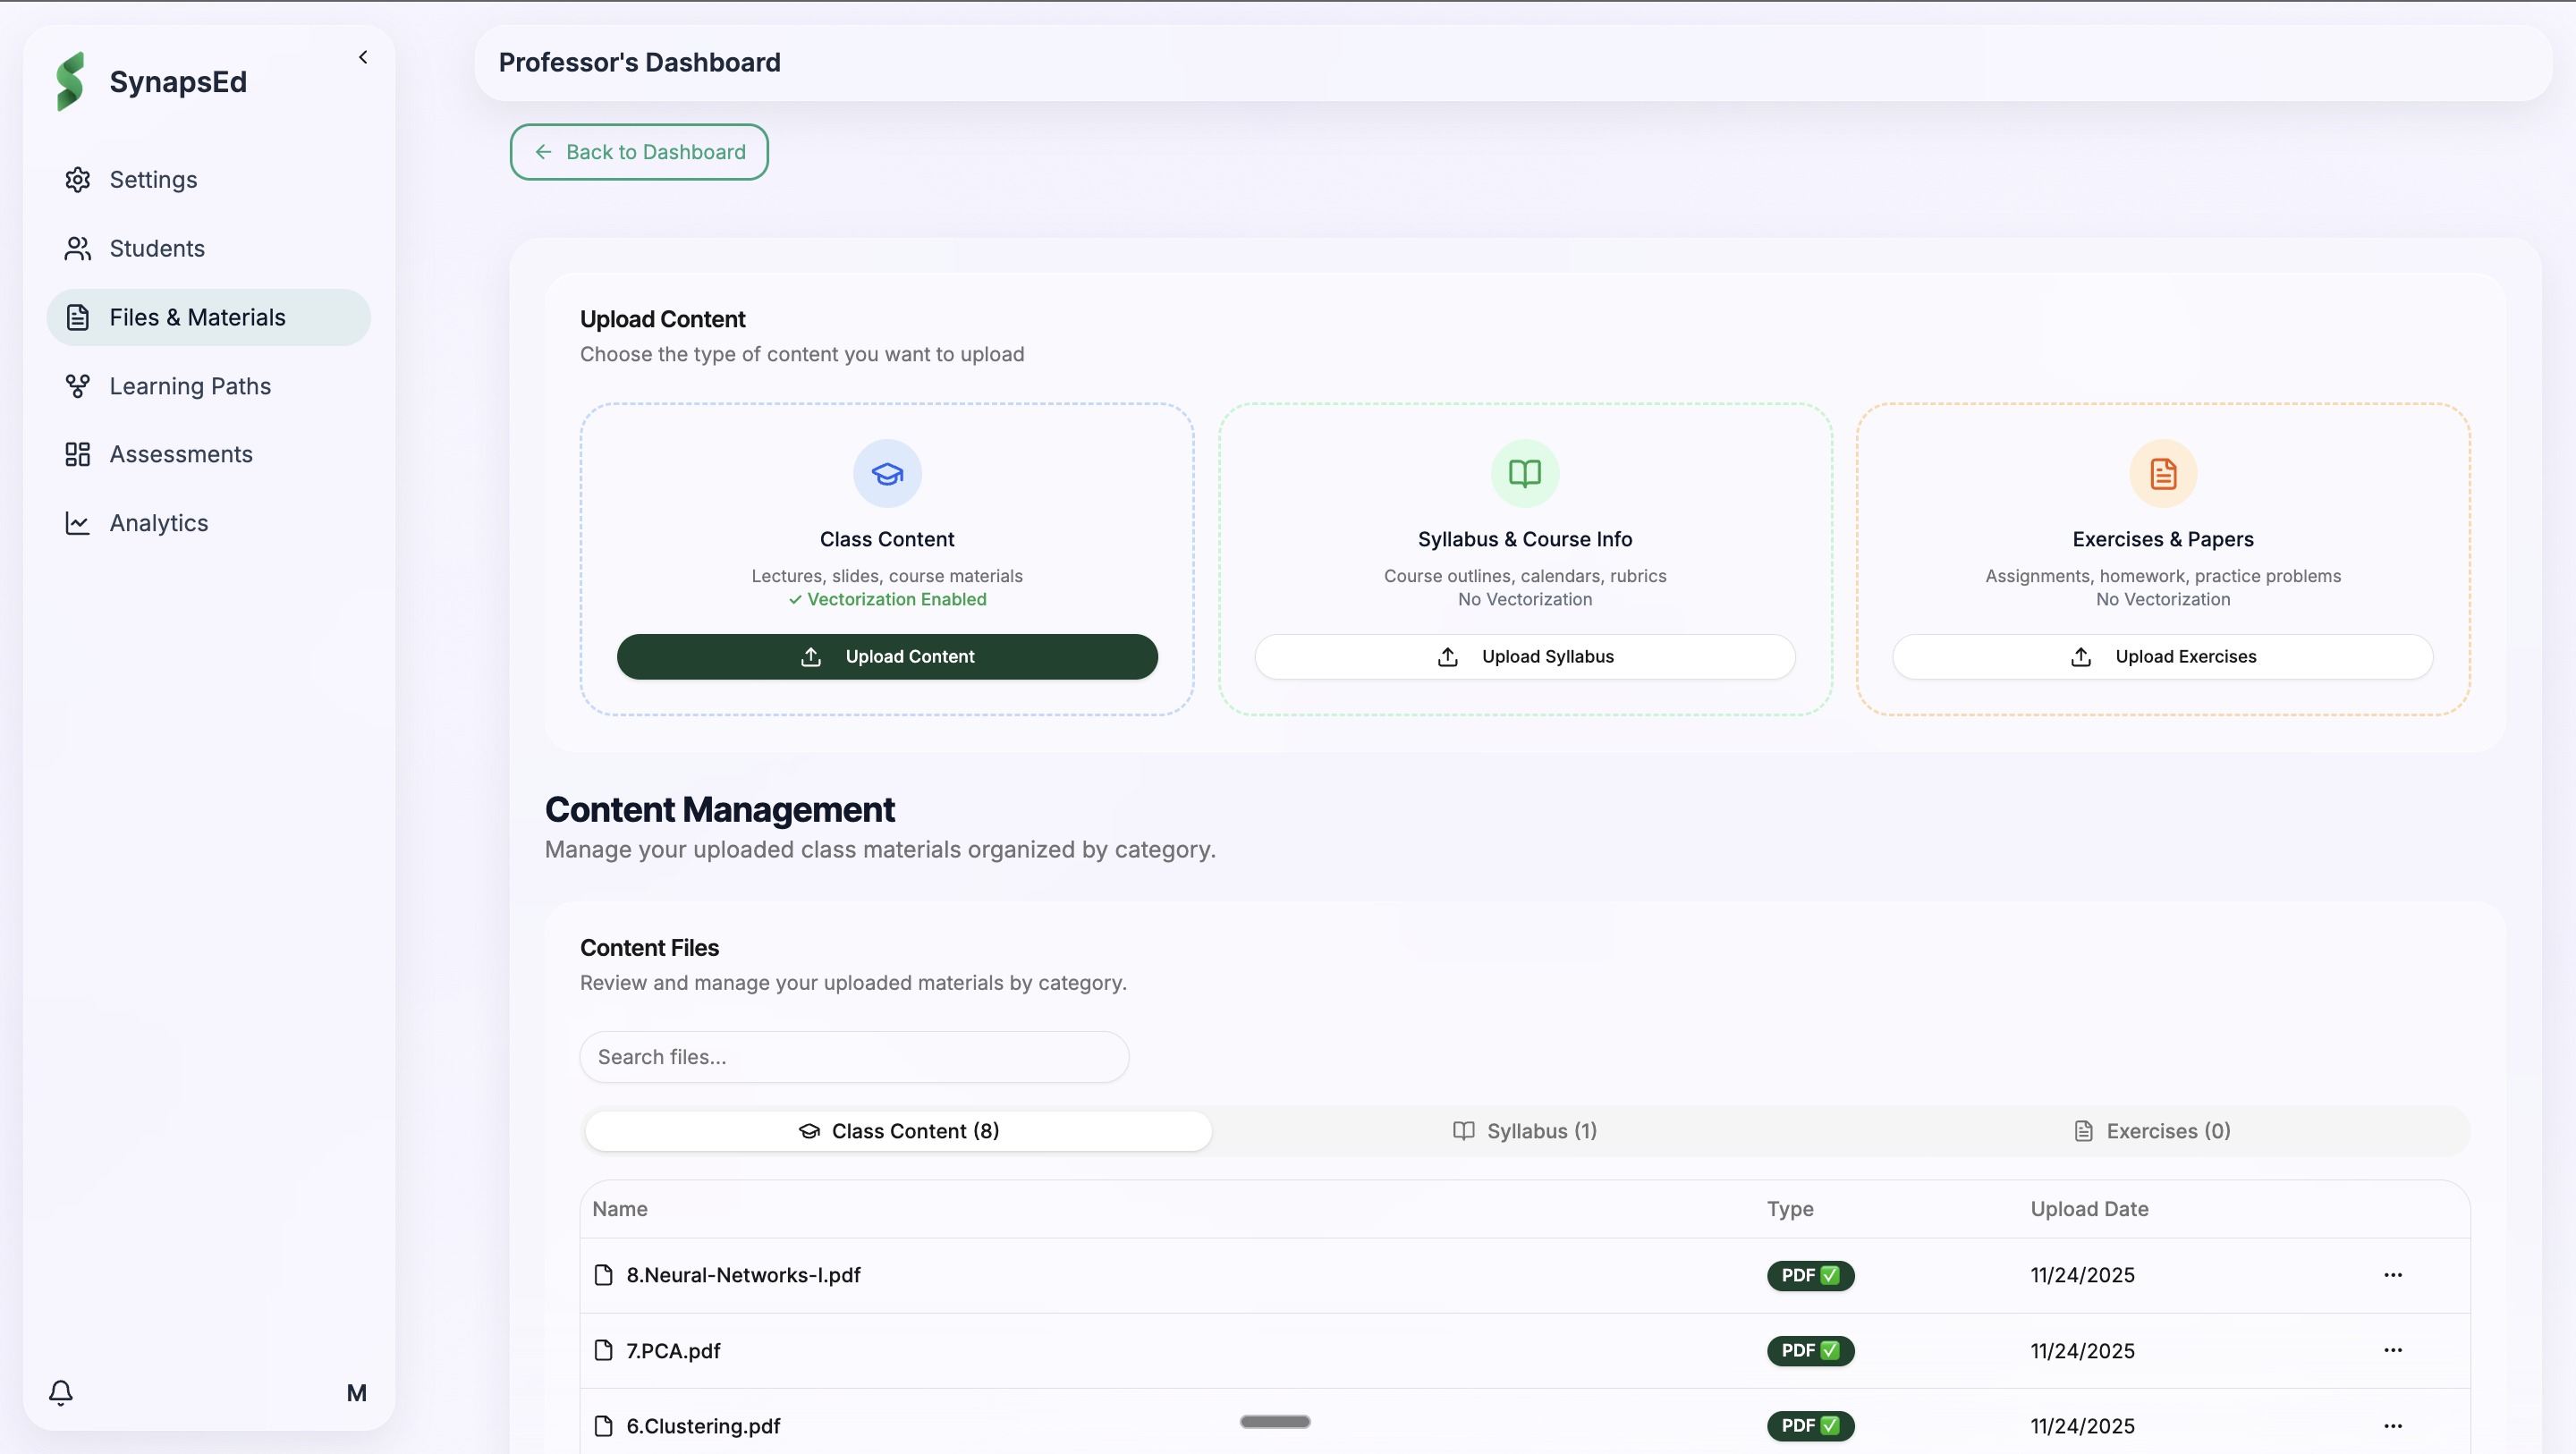
\includegraphics[width=0.8\columnwidth]{figures/instructor_upload.png}
\caption{Instructor content upload interface showing the drag-and-drop area for course materials with automatic background processing.}
\label{fig:instructor_upload}
\end{figure}

\textbf{Stage 2: Survey Generation and Customization.} Using the uploaded syllabus and course materials as context, instructors generate a diagnostic survey tailored to their specific course. By clicking "Generate with AI," the system produces 10-15 questions organized into five categories: prerequisite assessment, learning objectives readiness, assessment preparation, course-specific goals, and learning preferences. Instructors review the generated survey in draft mode, make any necessary edits to ensure alignment with their teaching philosophy, and publish it for student access. This survey serves as the foundation for understanding each student's prior knowledge, learning goals, and preferences. Figure~\ref{fig:survey_generation} illustrates the AI-assisted survey generation interface.

\begin{figure}[h]
\centering
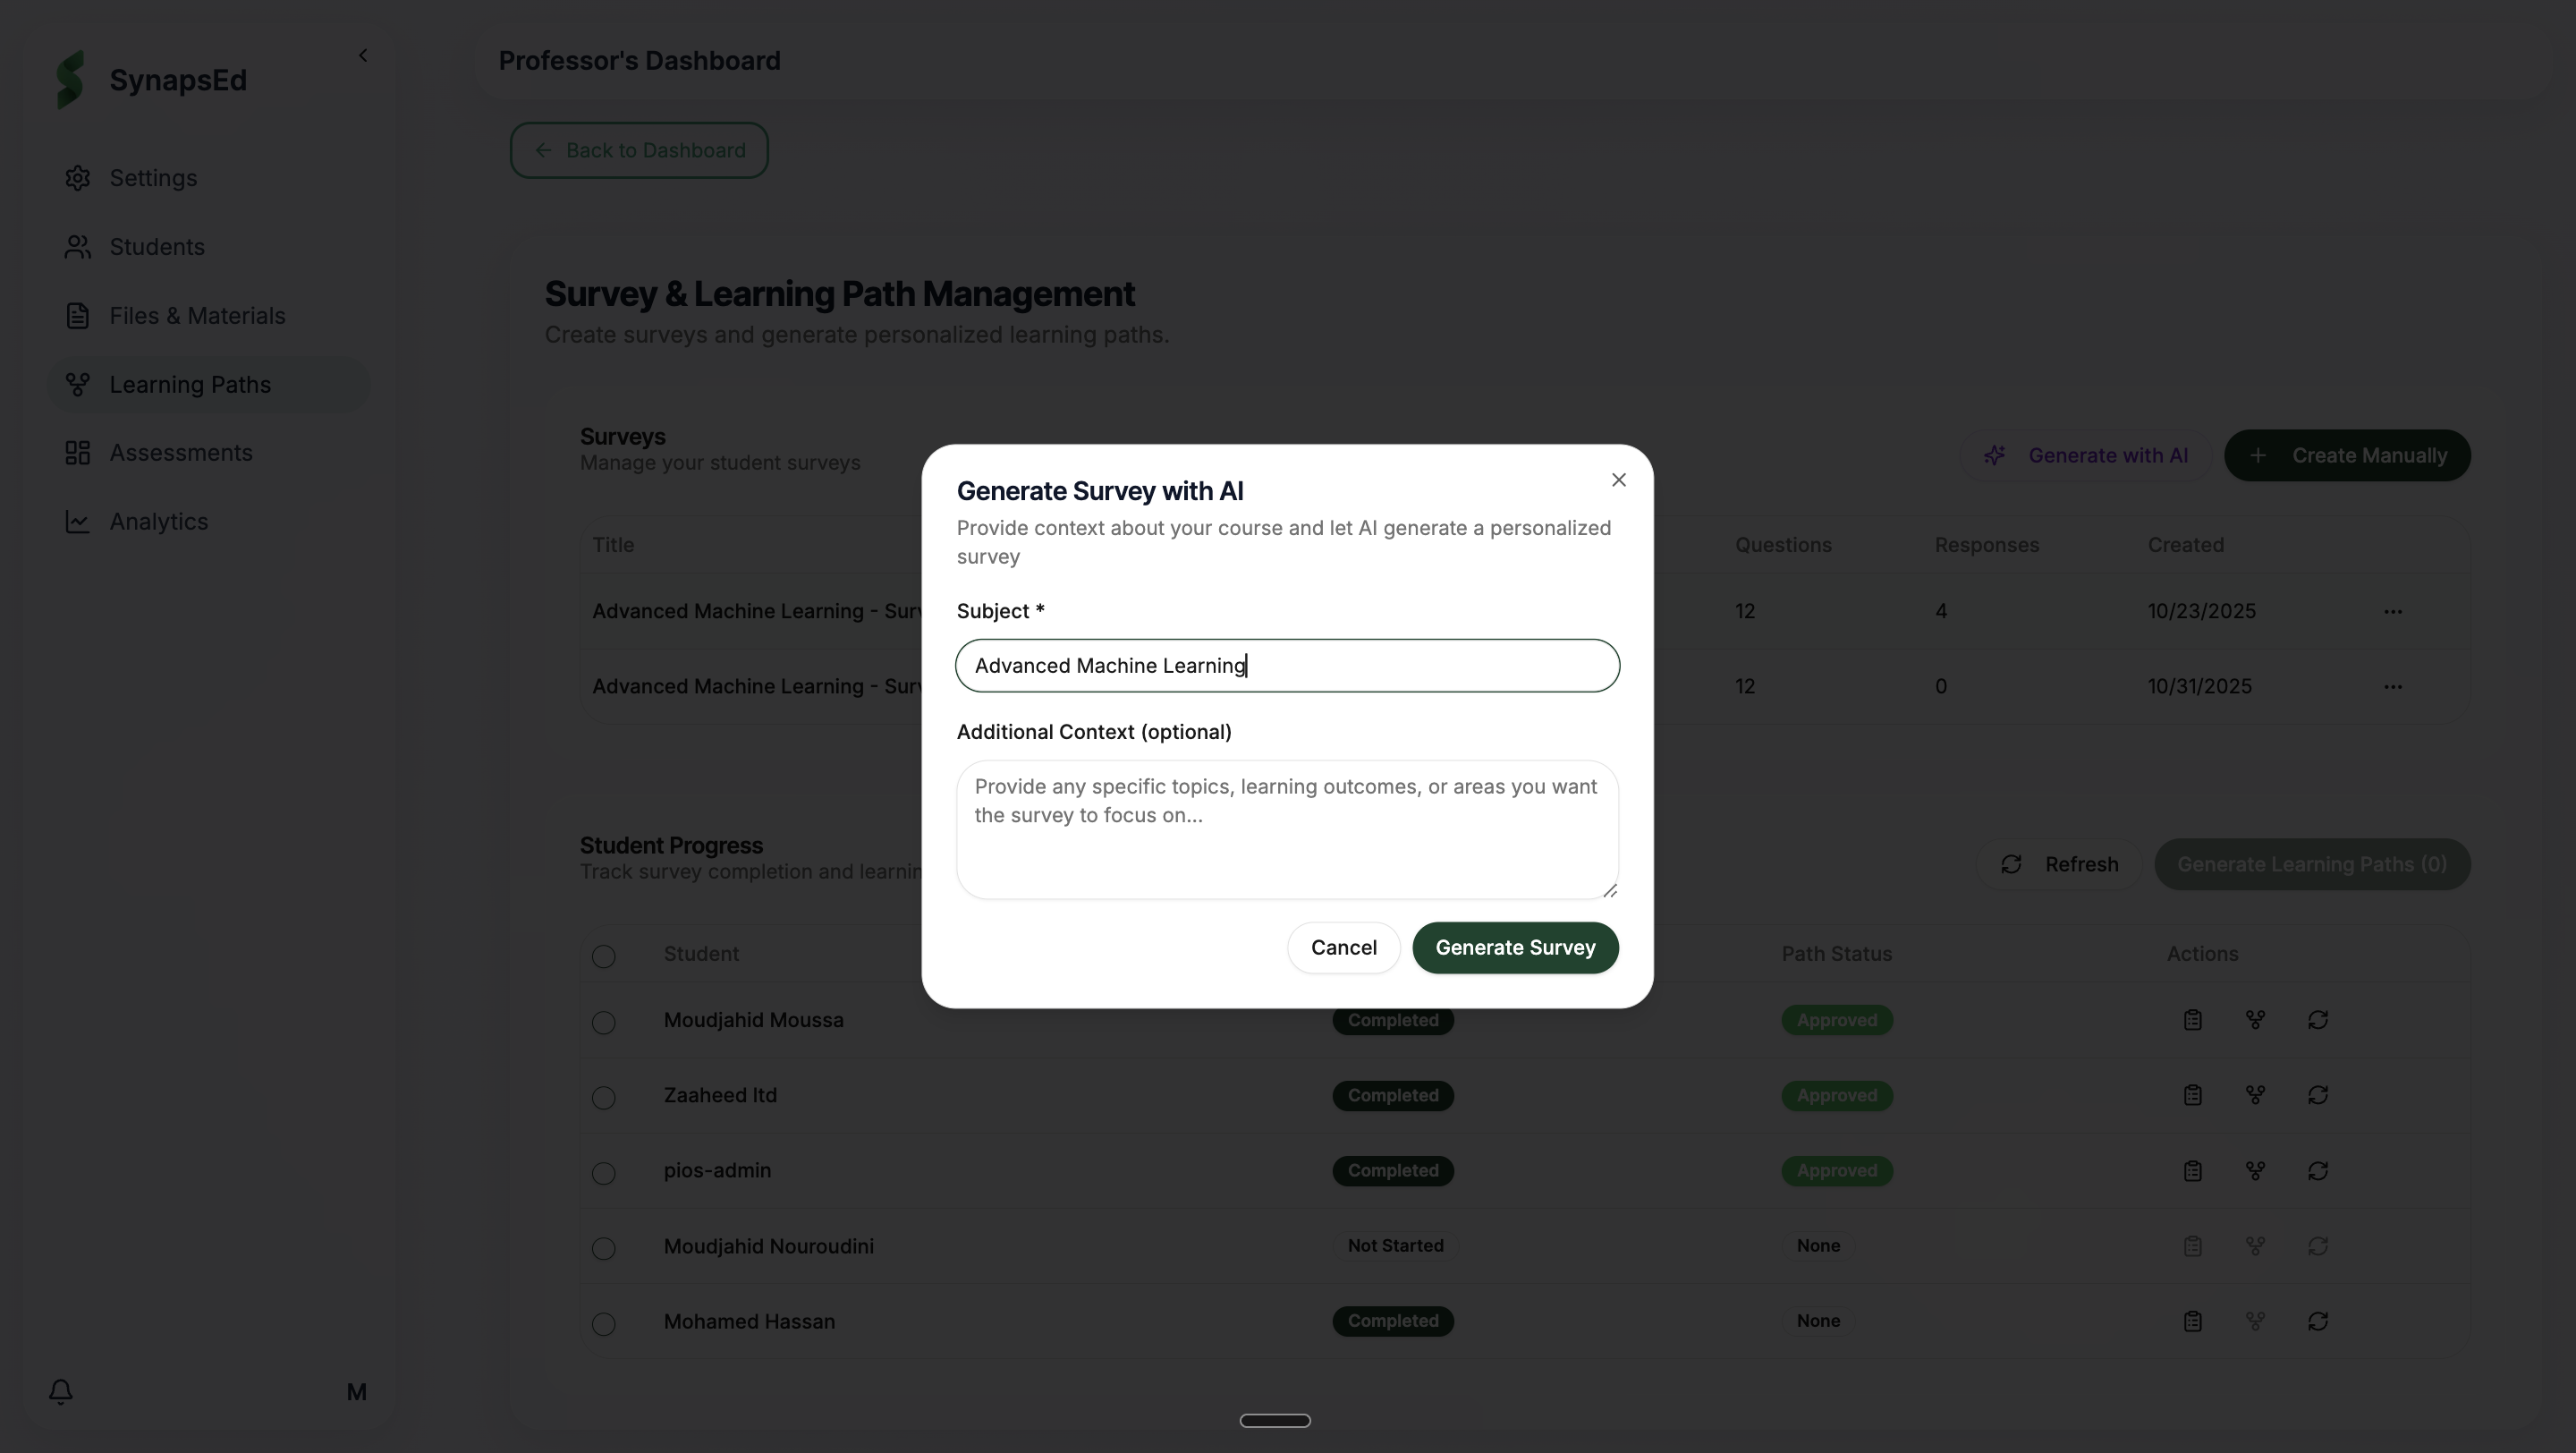
\includegraphics[width=0.8\columnwidth]{figures/survey_generation.png}
\caption{Survey generation interface where instructors can generate, review, and customize diagnostic surveys using AI assistance.}
\label{fig:survey_generation}
\end{figure}

\textbf{Stage 3: Pathway Review and Approval.} Once students complete the survey, instructors trigger pathway generation for each student. The system generates personalized learning pathways consisting of 10-14 sequential nodes, each representing a focused learning objective with associated resources, prerequisites, and assessment opportunities. Instructors review each generated pathway through a structured interface and can take three actions: approve the pathway to make it visible to the student, reject it with feedback if it does not meet pedagogical standards, or regenerate it with additional constraints or focus areas. This approval workflow ensures that every student-facing pathway has been vetted by the instructor before deployment. Figure~\ref{fig:pathway_review} shows the pathway review interface with approval options.

\begin{figure}[h]
\centering
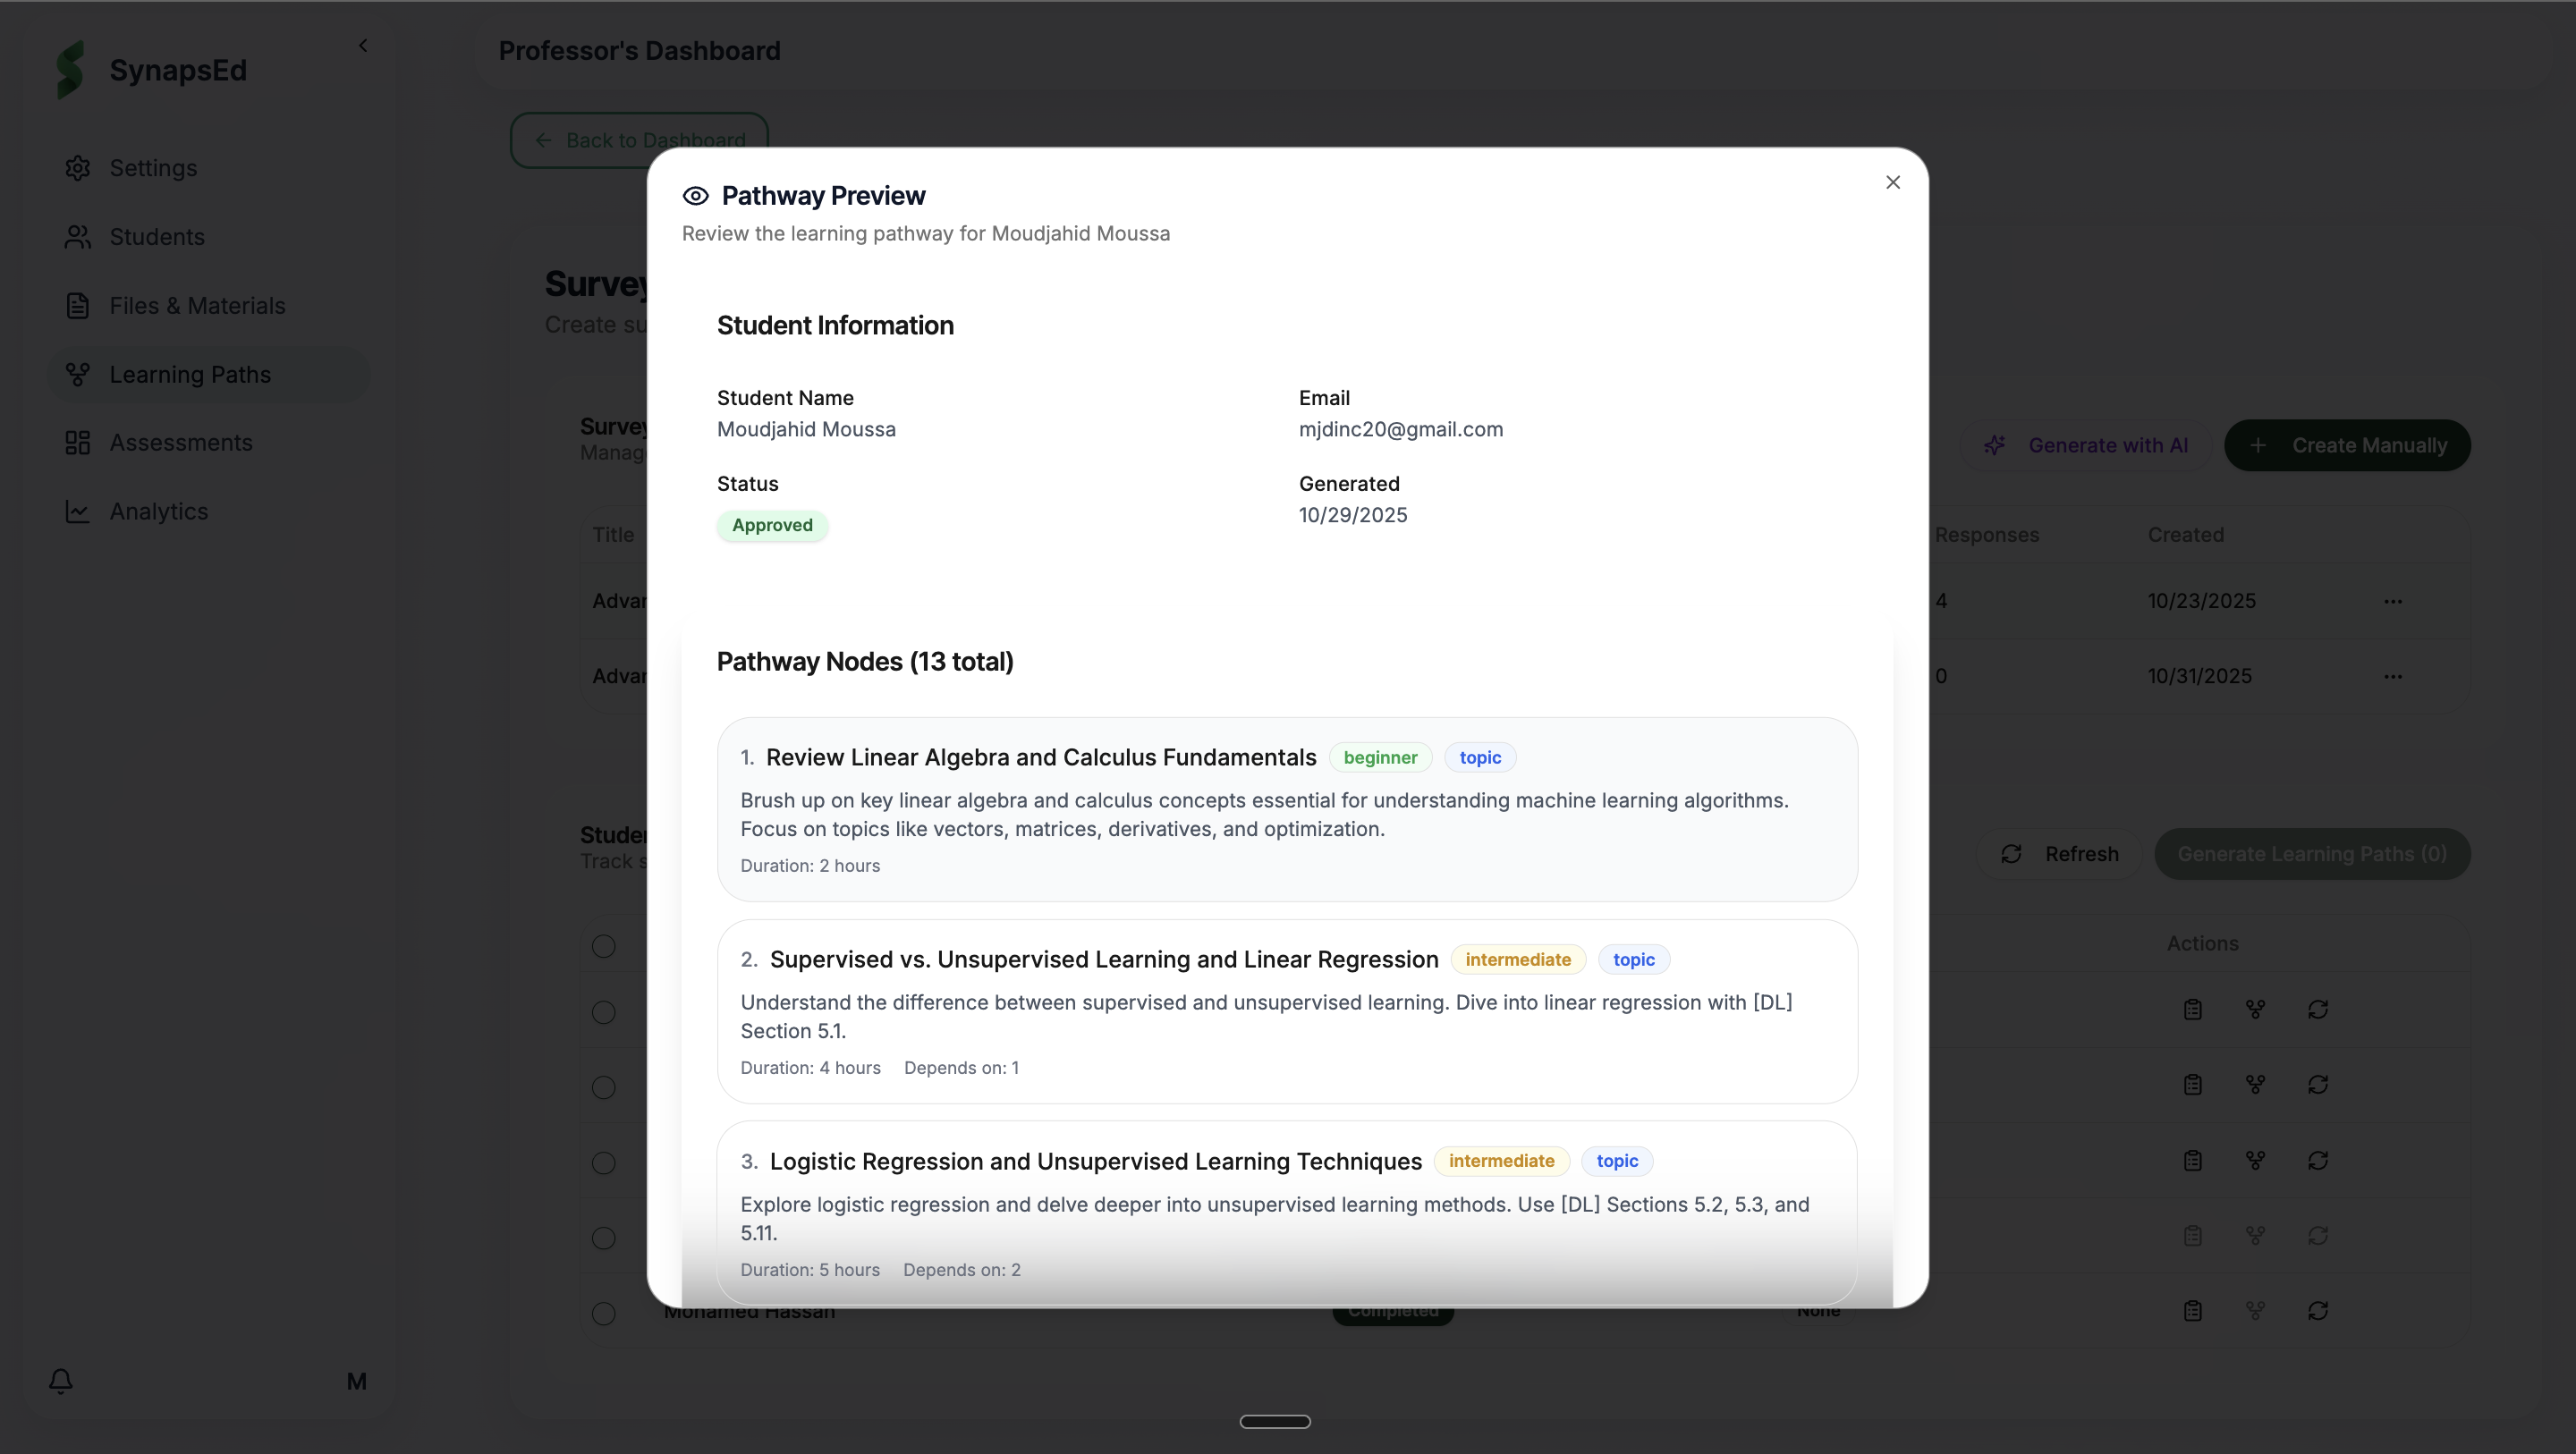
\includegraphics[width=0.8\columnwidth]{figures/pathway_review.png}
\caption{Pathway review interface showing the sequential learning nodes and instructor approval controls (approve, reject, regenerate).}
\label{fig:pathway_review}
\end{figure}

\textbf{Stage 4: Monitoring and Intervention.} Throughout the semester, instructors access an aggregate analytics dashboard showing class-level insights including common challenges, content areas where students struggle, and overall progress patterns. This dashboard does not expose individual student data but instead surfaces actionable patterns that inform instructional decisions. Instructors can identify which concepts require additional lecture time or which resources need refinement based on aggregate student interactions with the intelligent tutoring agent. Figure~\ref{fig:instructor_dashboard} presents the aggregate analytics dashboard.

\begin{figure}[h]
\centering
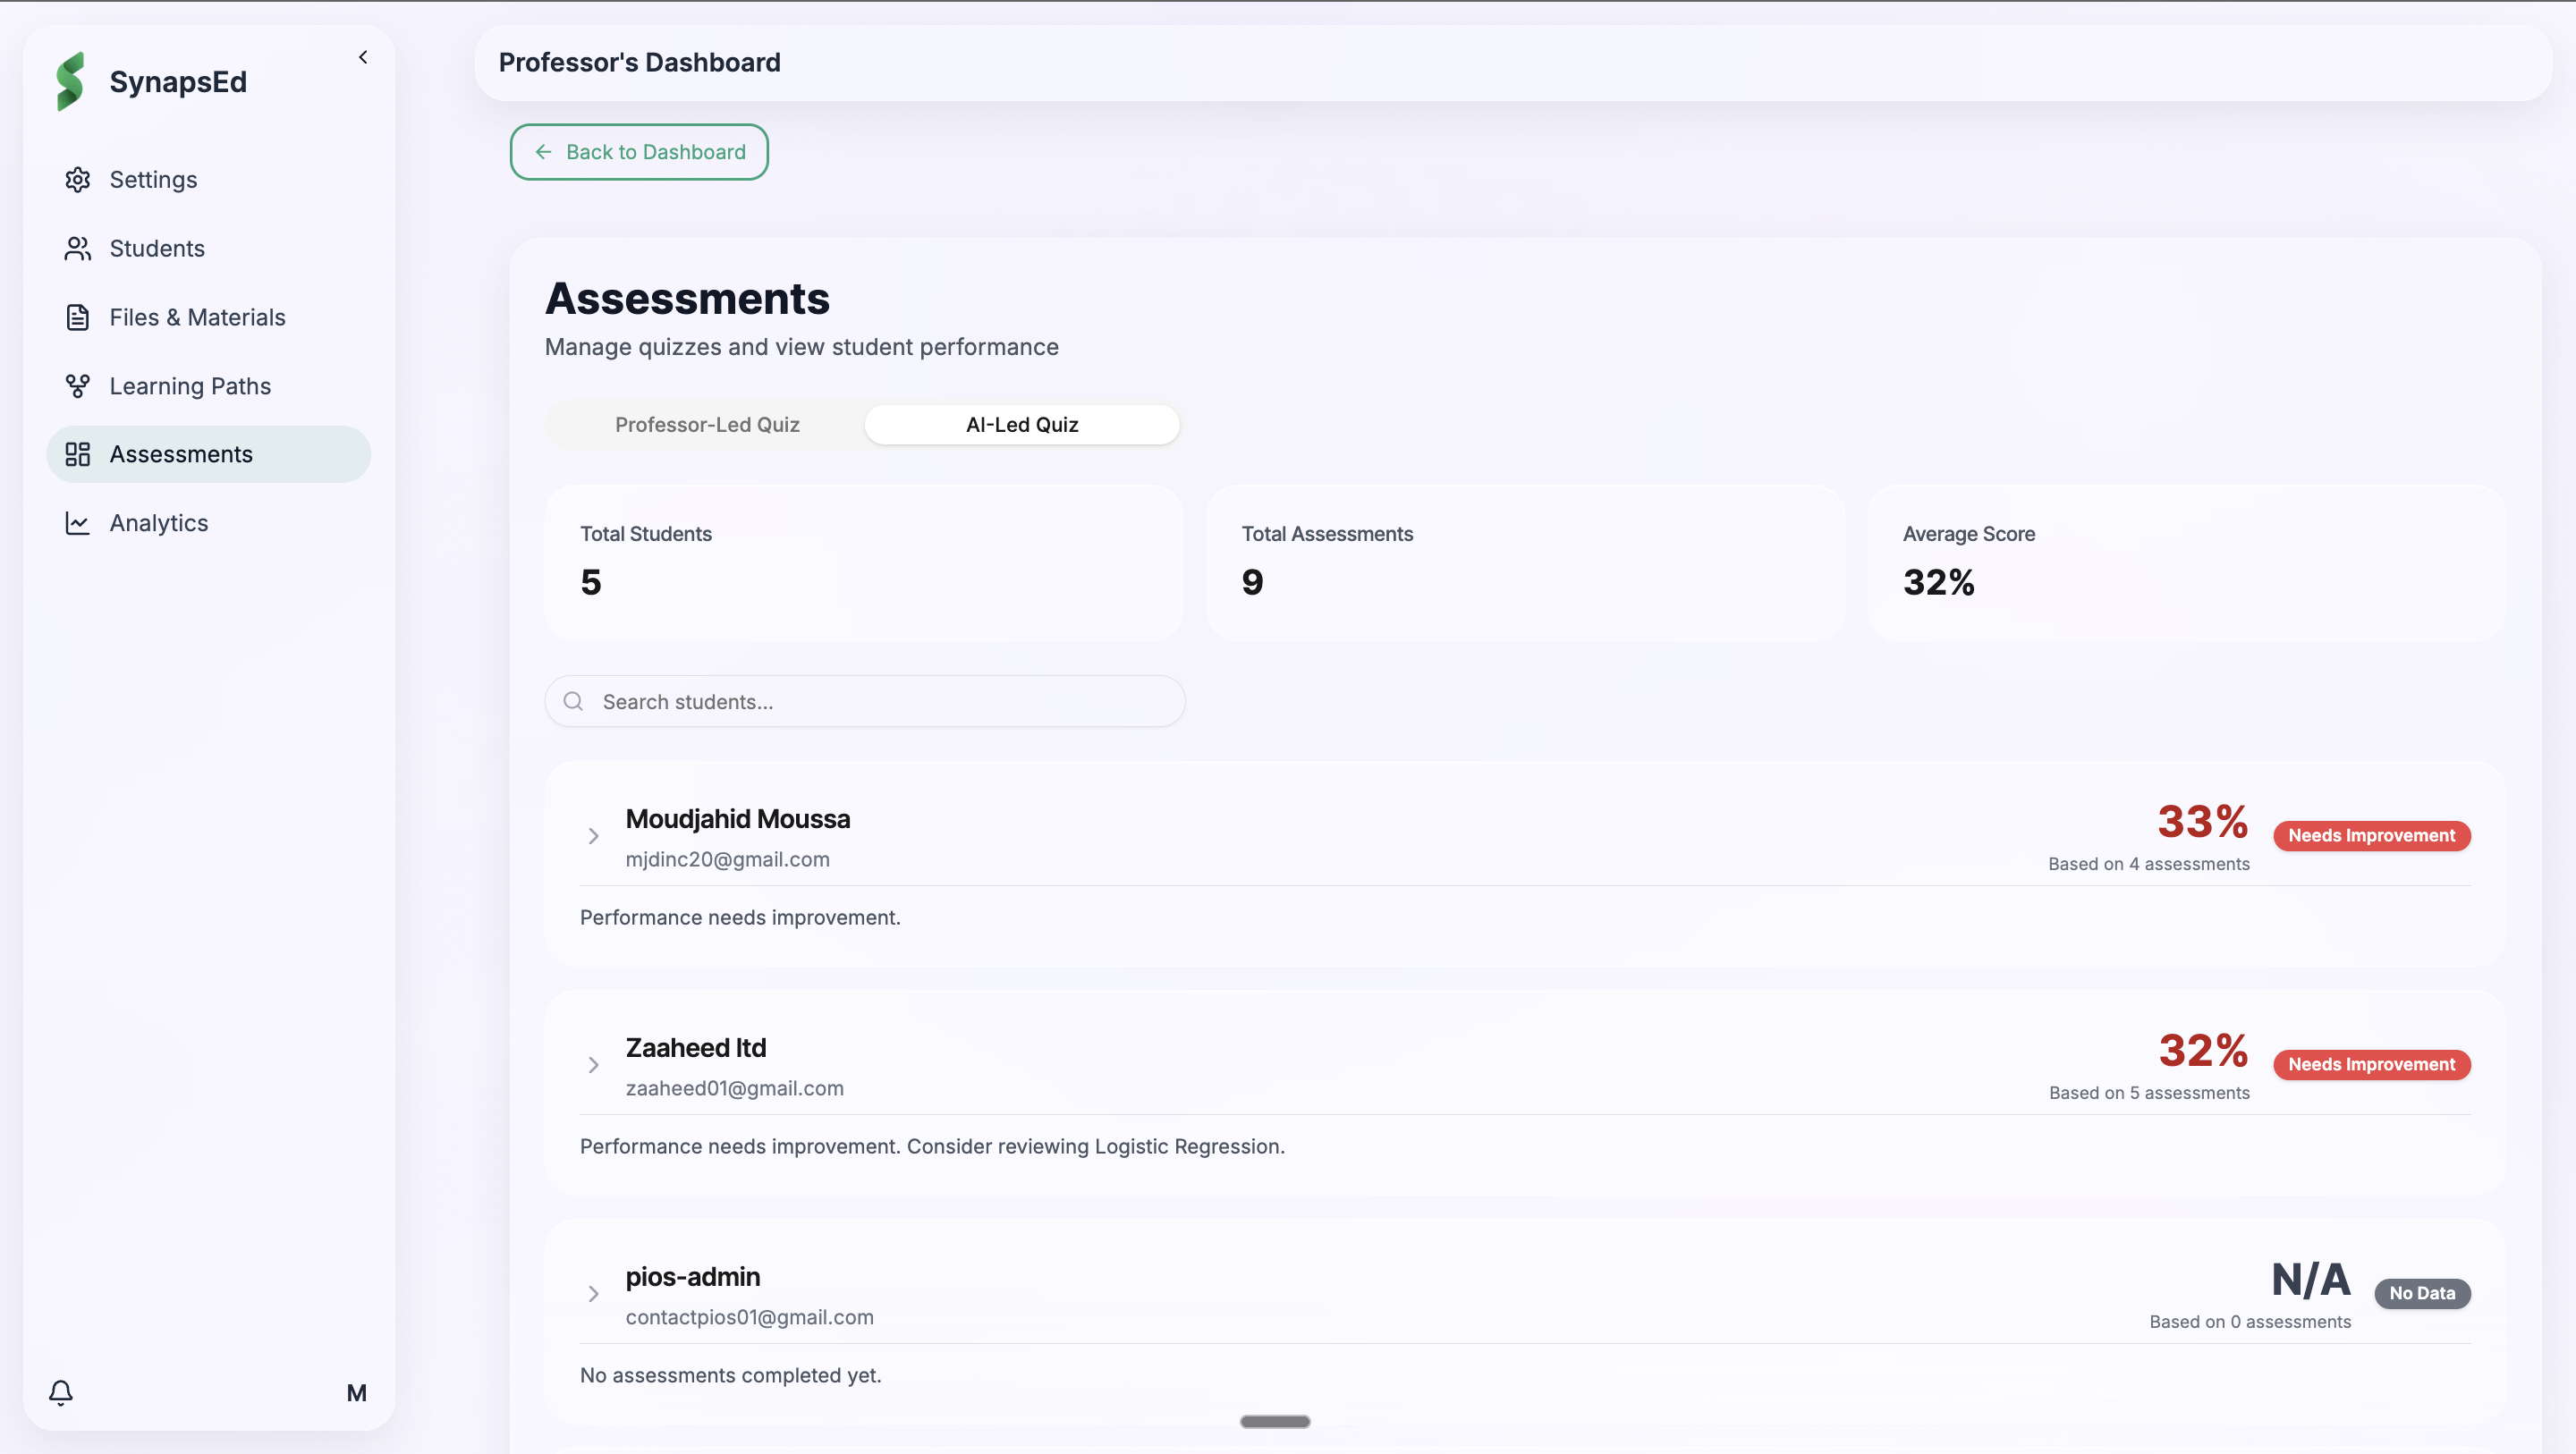
\includegraphics[width=0.8\columnwidth]{figures/instructor_dashboard.png}
\caption{Instructor analytics dashboard displaying aggregate class-level insights about student progress and common challenges.}
\label{fig:instructor_dashboard}
\end{figure}

\subsubsection{The Student Workflow}

Students interact with SynapsEd through a four-stage learning journey designed to provide personalized guidance while maintaining transparency:

\textbf{Stage 1: Onboarding and Assessment.} Upon joining a course, students complete the instructor-created diagnostic survey. This survey asks about their prior knowledge of prerequisite concepts, readiness for specific learning objectives, preferred assessment methods, personal learning goals aligned with course content, and learning style preferences. The survey typically takes 10-15 minutes to complete and provides the system with the information needed to tailor subsequent recommendations. Figure~\ref{fig:student_survey} shows the student survey interface.

\begin{figure}[h]
\centering
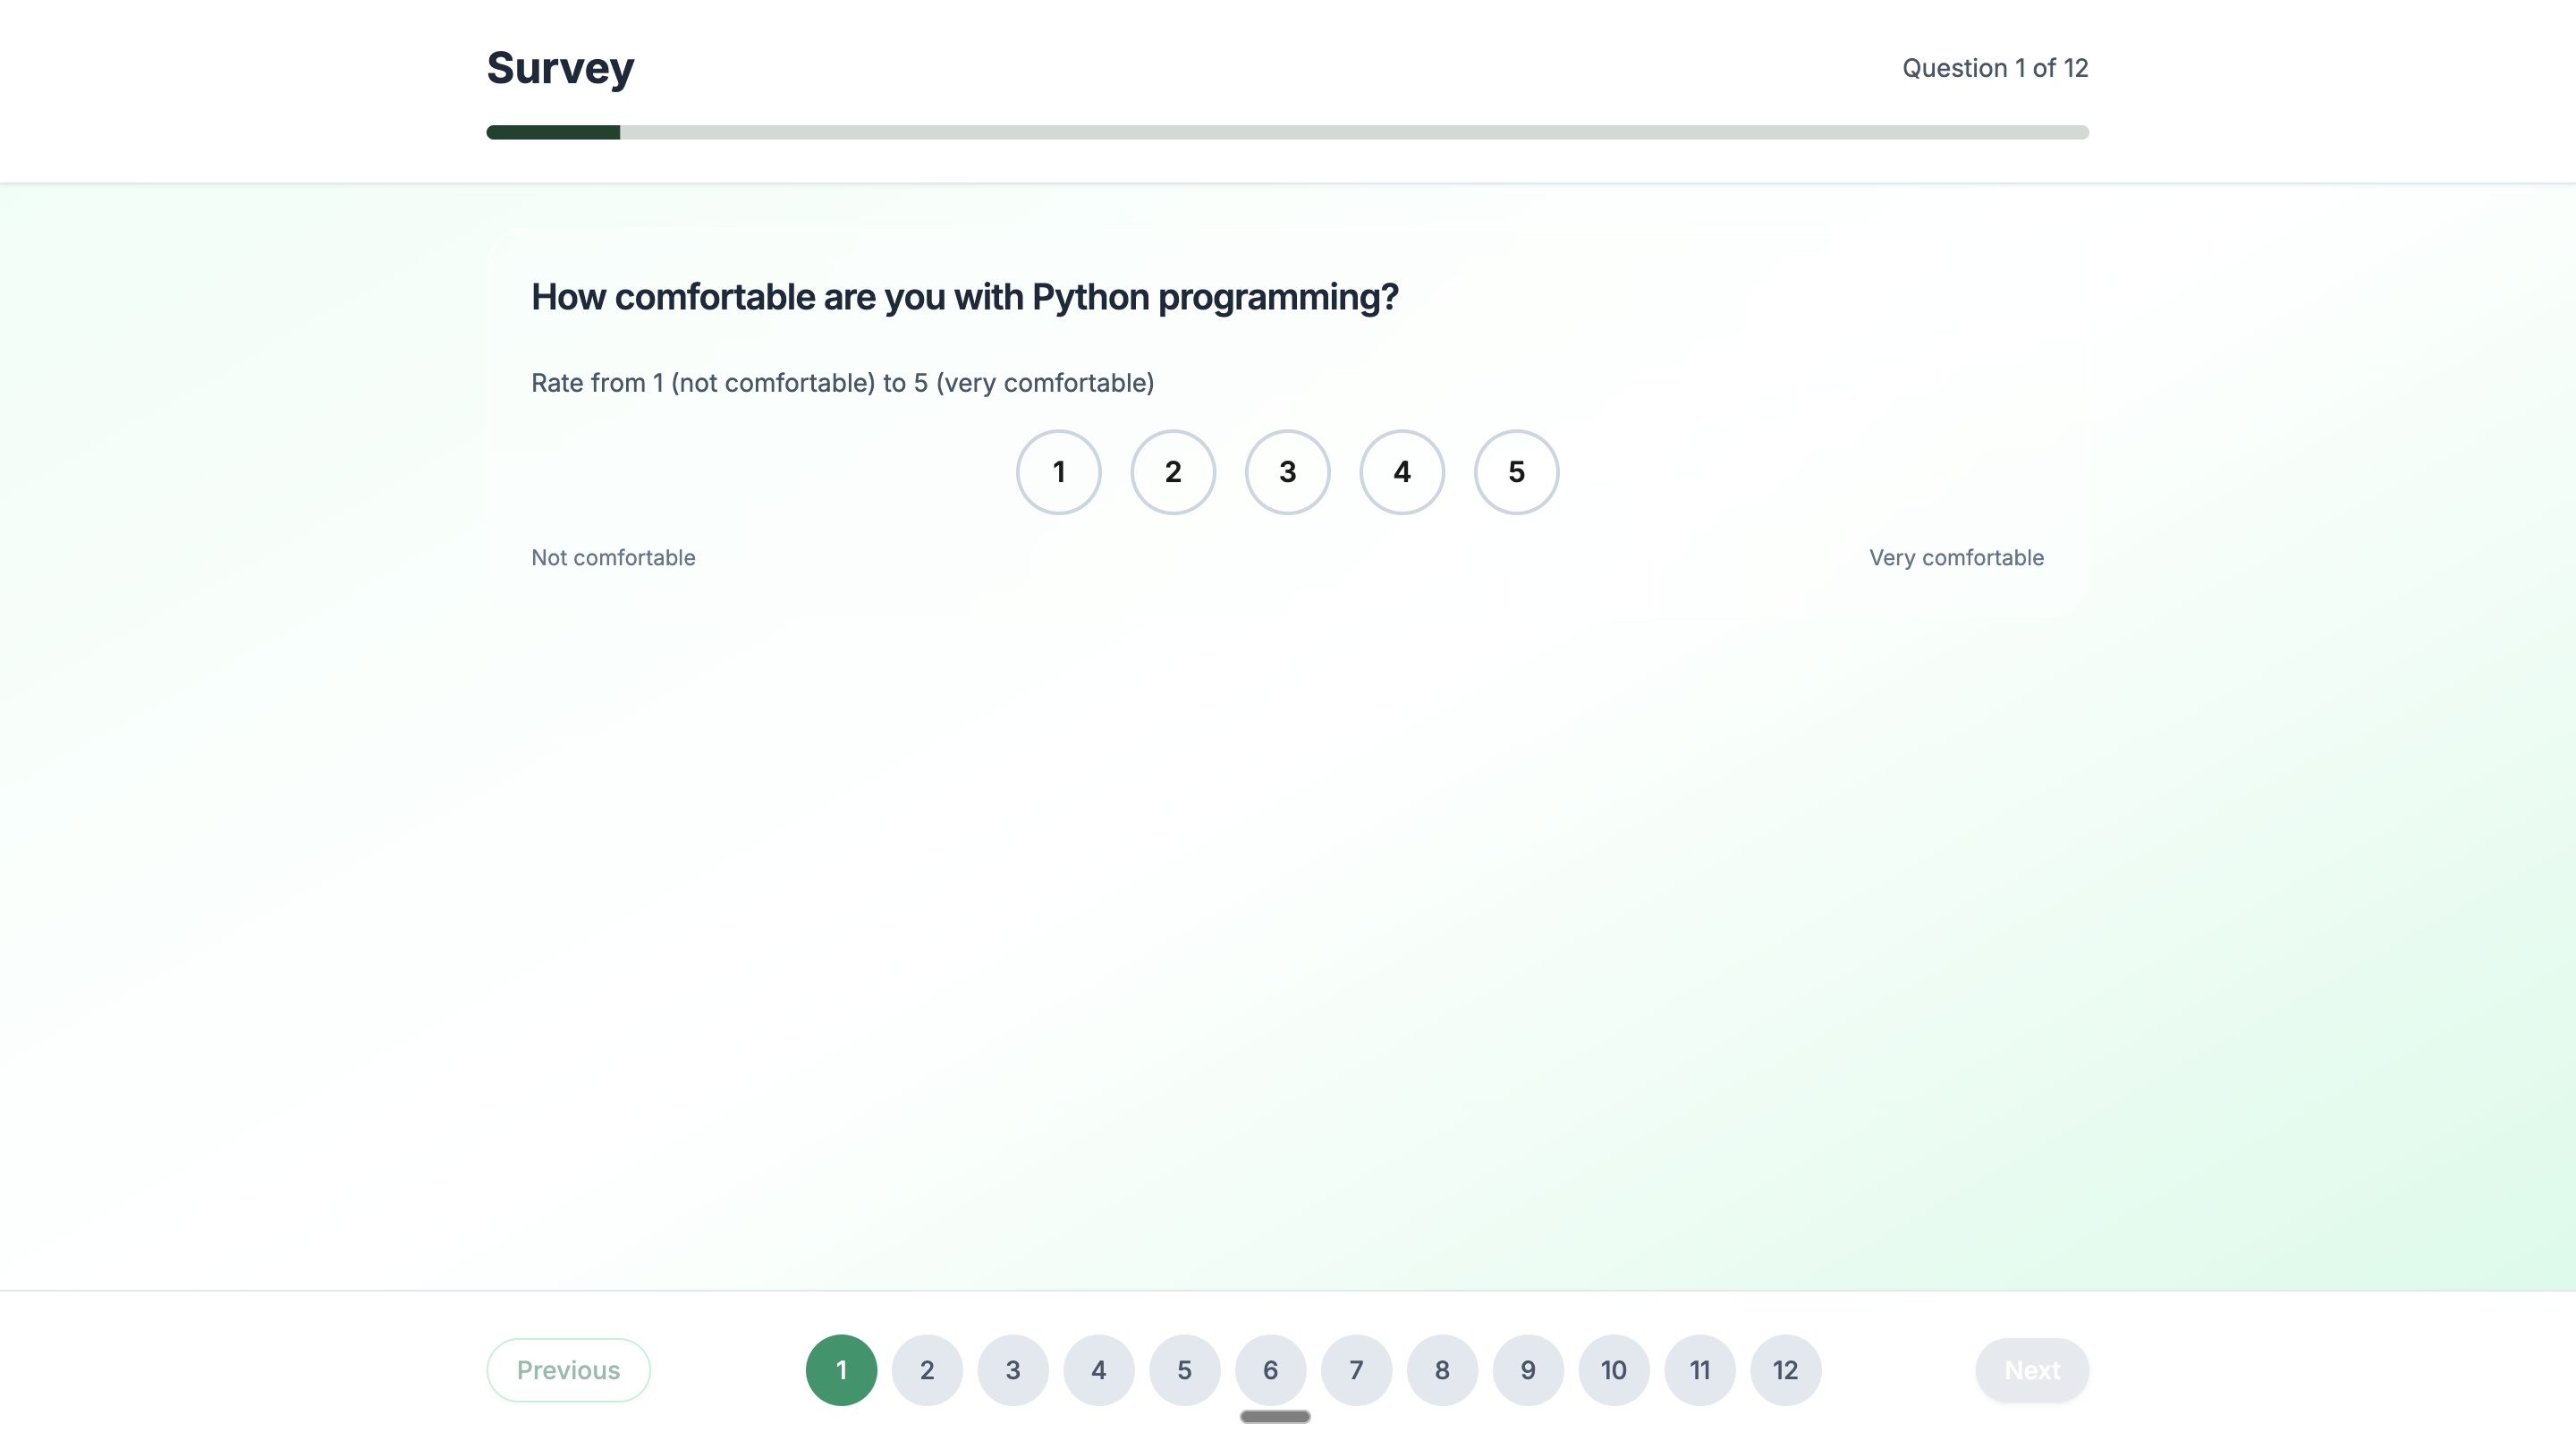
\includegraphics[width=0.8\columnwidth]{figures/student_survey.png}
\caption{Student diagnostic survey interface with course-specific questions about prior knowledge, goals, and learning preferences.}
\label{fig:student_survey}
\end{figure}

\textbf{Stage 2: Pathway Reception and Exploration.} After the instructor approves their pathway, students receive access to their personalized learning journey. The pathway is presented as a visual sequence of nodes, each representing a focused learning objective. Students can view the entire pathway structure, understand the prerequisite relationships between nodes, and see how their pathway aligns with course learning objectives. Each node displays its title, learning objectives, estimated time commitment, and Bloom's taxonomy level, providing transparency about what they will learn and why. Figure~\ref{fig:student_pathway} illustrates the student's personalized pathway visualization.

\begin{figure}[h]
\centering
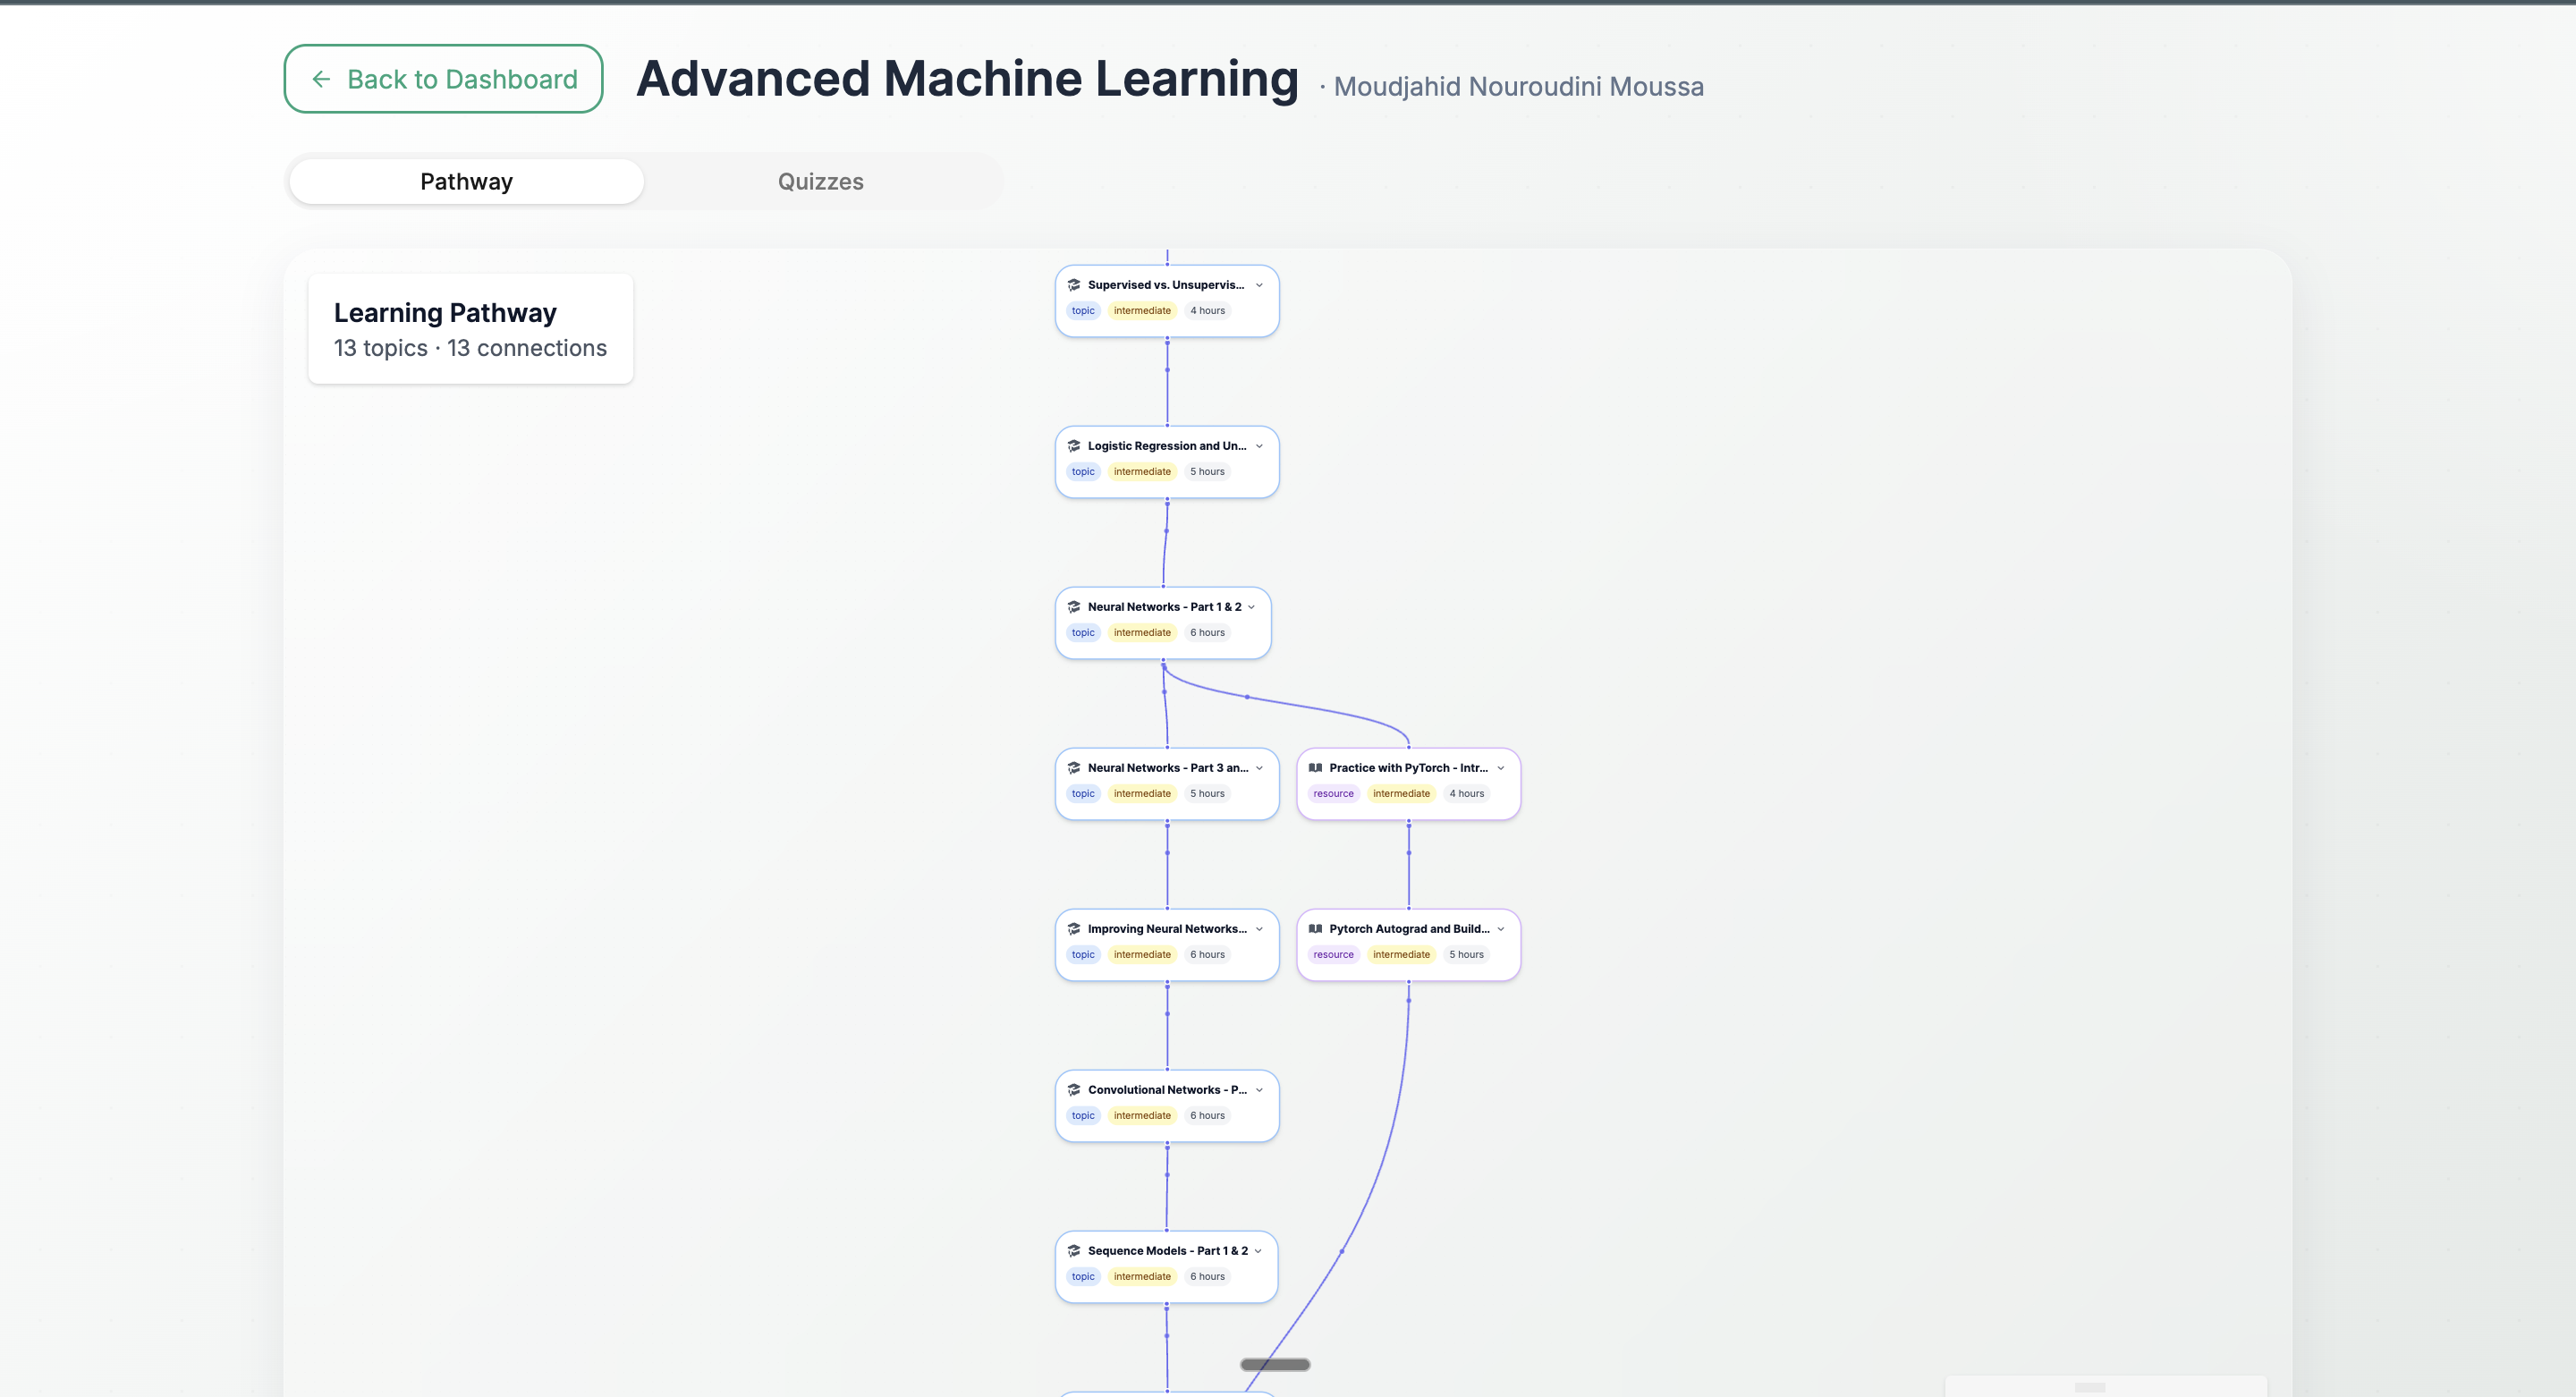
\includegraphics[width=0.8\columnwidth]{figures/student_pathway.png}
\caption{Student pathway interface showing the visual sequence of learning nodes with prerequisite relationships and progress tracking.}
\label{fig:student_pathway}
\end{figure}

\textbf{Stage 3: Interactive Learning and Tutoring.} As students progress through their pathway, they engage with an intelligent tutoring agent that uses the Socratic method to guide learning. When entering a new node, the agent introduces the topic through thought-provoking questions rather than direct instruction, encouraging active engagement. Students can ask questions, request clarification, or explore related concepts through a chat interface. The agent dynamically retrieves relevant passages from the instructor's uploaded materials using semantic search, ensuring all responses are grounded in course content. The agent can also generate formative assessments (quizzes, practice problems) on demand to check understanding. All agent responses include source attribution, allowing students to navigate back to the original course materials for deeper study. Figure~\ref{fig:tutoring_interface} shows the interactive tutoring chat interface with source attribution.

\begin{figure}[h]
\centering
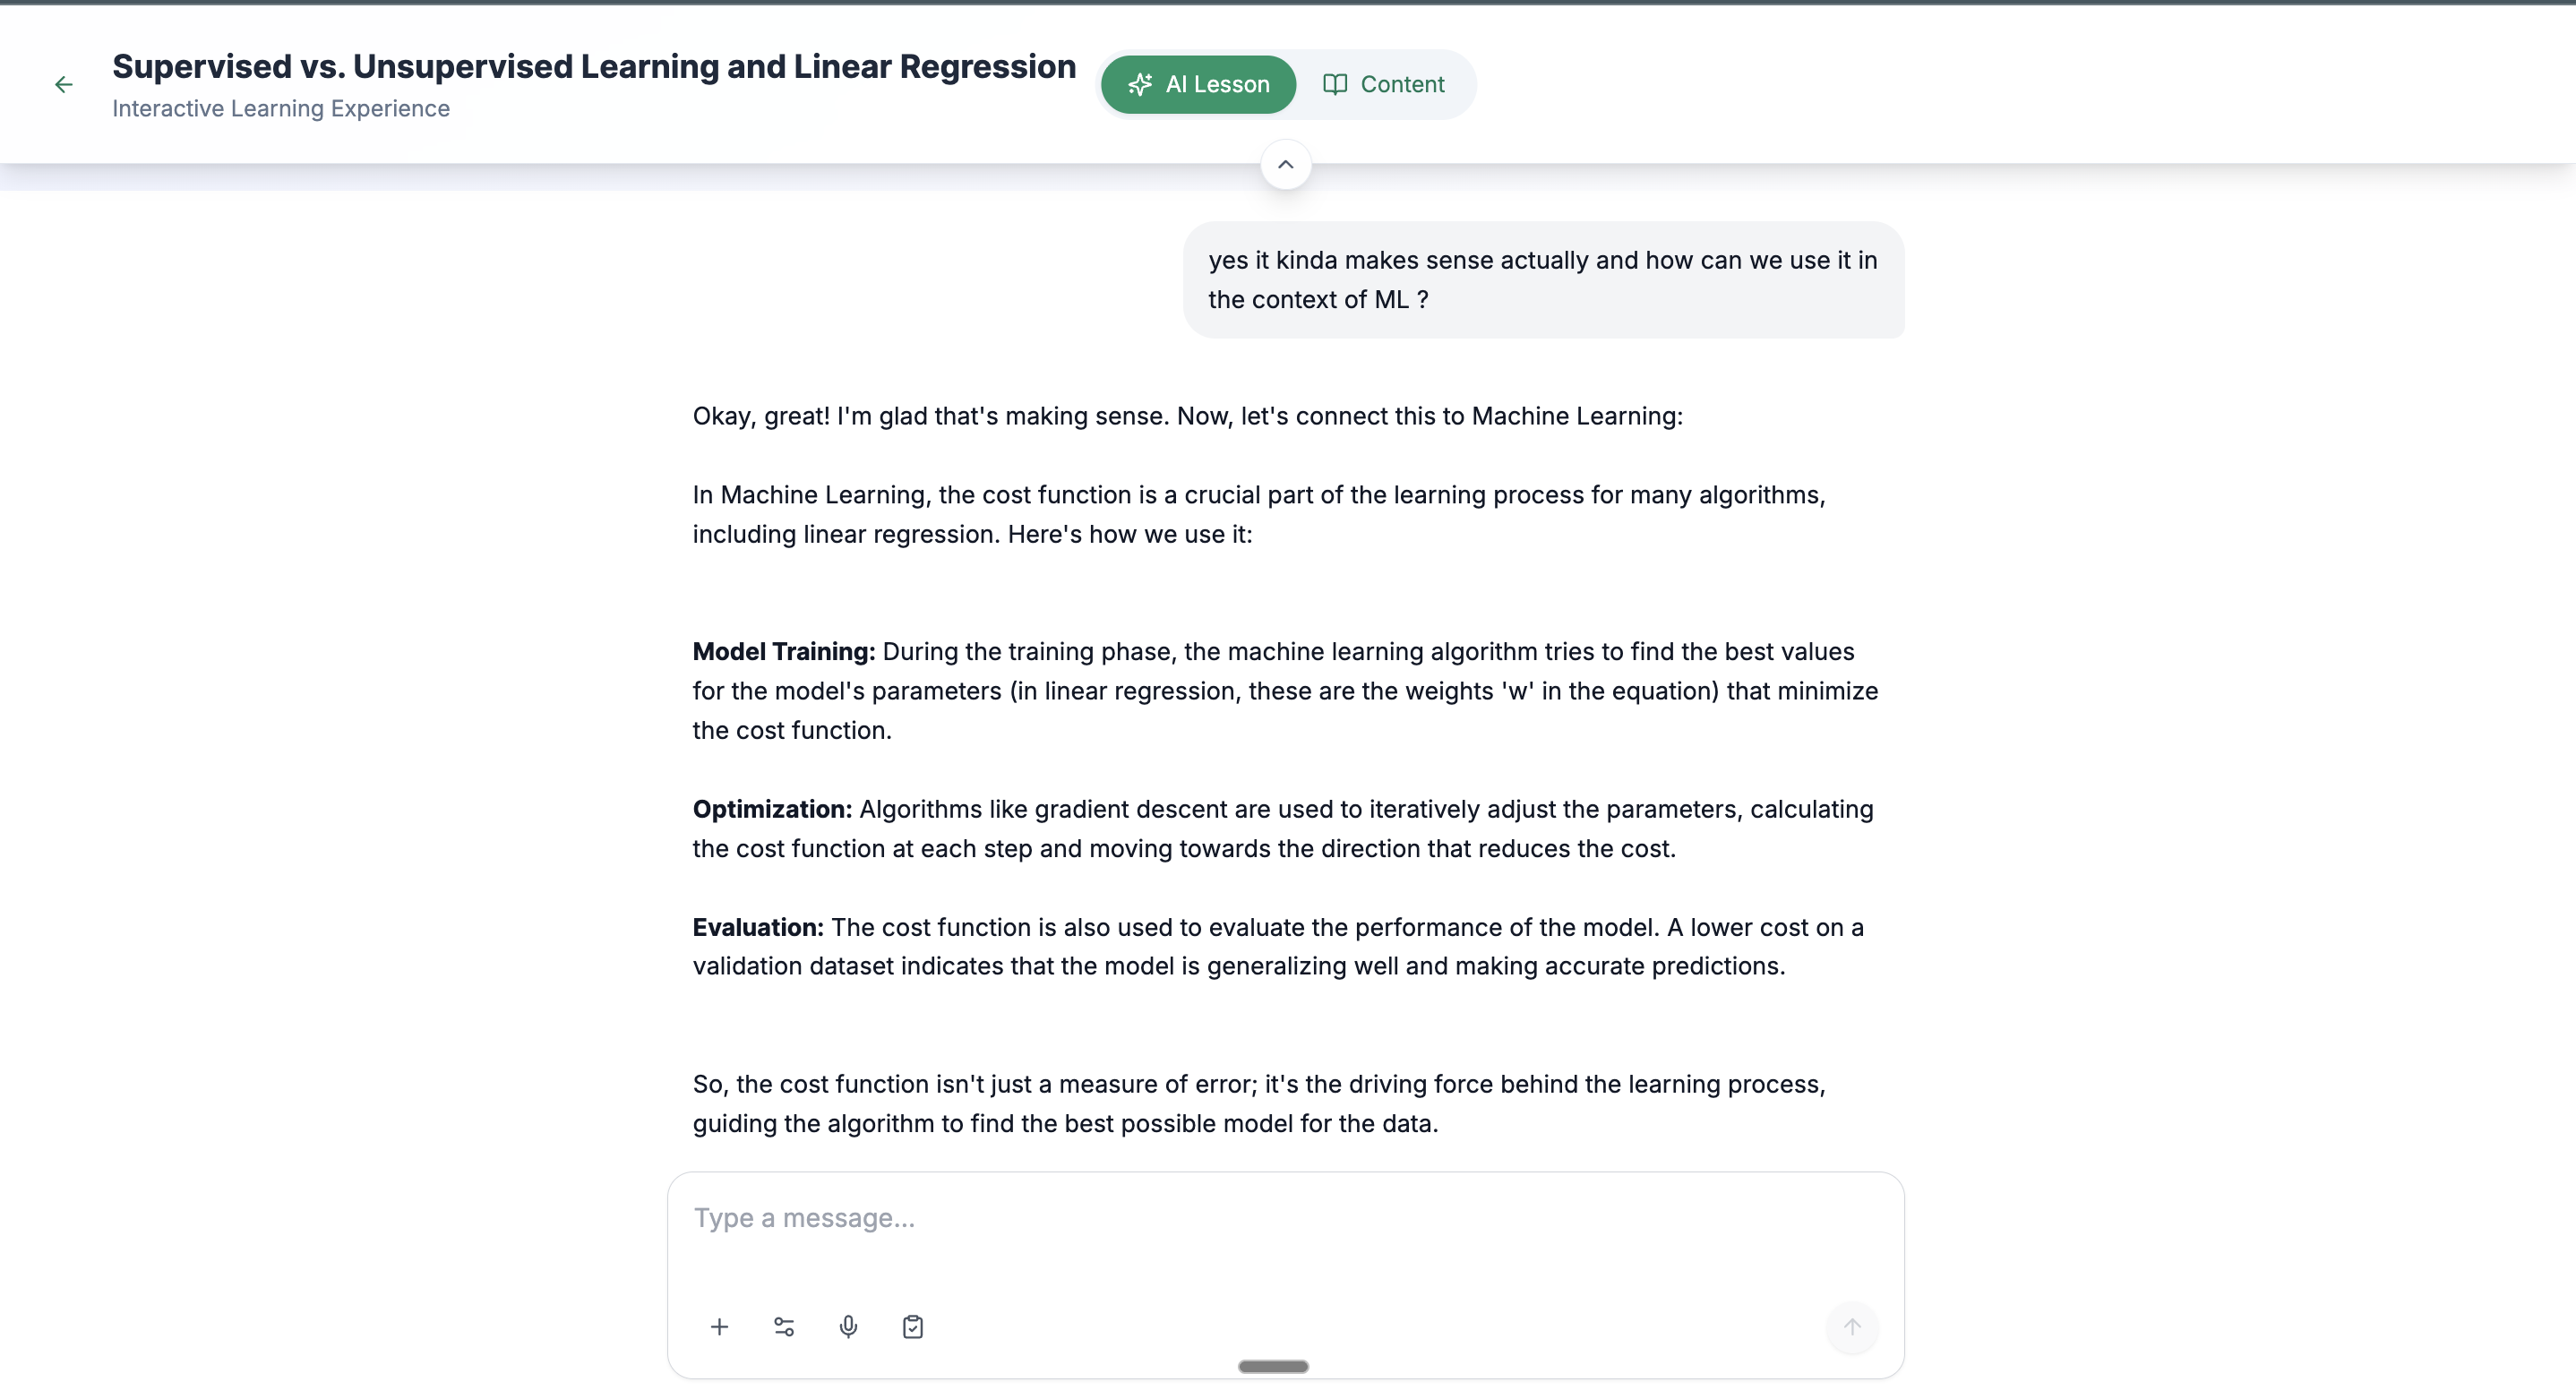
\includegraphics[width=0.8\columnwidth]{figures/tutoring_interface.png}
\caption{Interactive tutoring interface showing the Socratic-method chat, dynamic content retrieval, and source attribution to course materials.}
\label{fig:tutoring_interface}
\end{figure}

\textbf{Stage 4: Adaptive Progression.} As students interact with content and complete assessments, the system tracks their performance and adjusts subsequent recommendations accordingly. If a student demonstrates strong understanding of a concept, the system may suggest more advanced materials or accelerate progression. If a student struggles with a concept, the system may recommend additional prerequisite review or alternative explanations. This adaptation happens transparently, students receive explanations for why certain content is recommended and can see how their performance influences the pathway. Figure~\ref{fig:adaptive_feedback} demonstrates how the system provides adaptive recommendations based on student performance.

\begin{figure}[h]
\centering
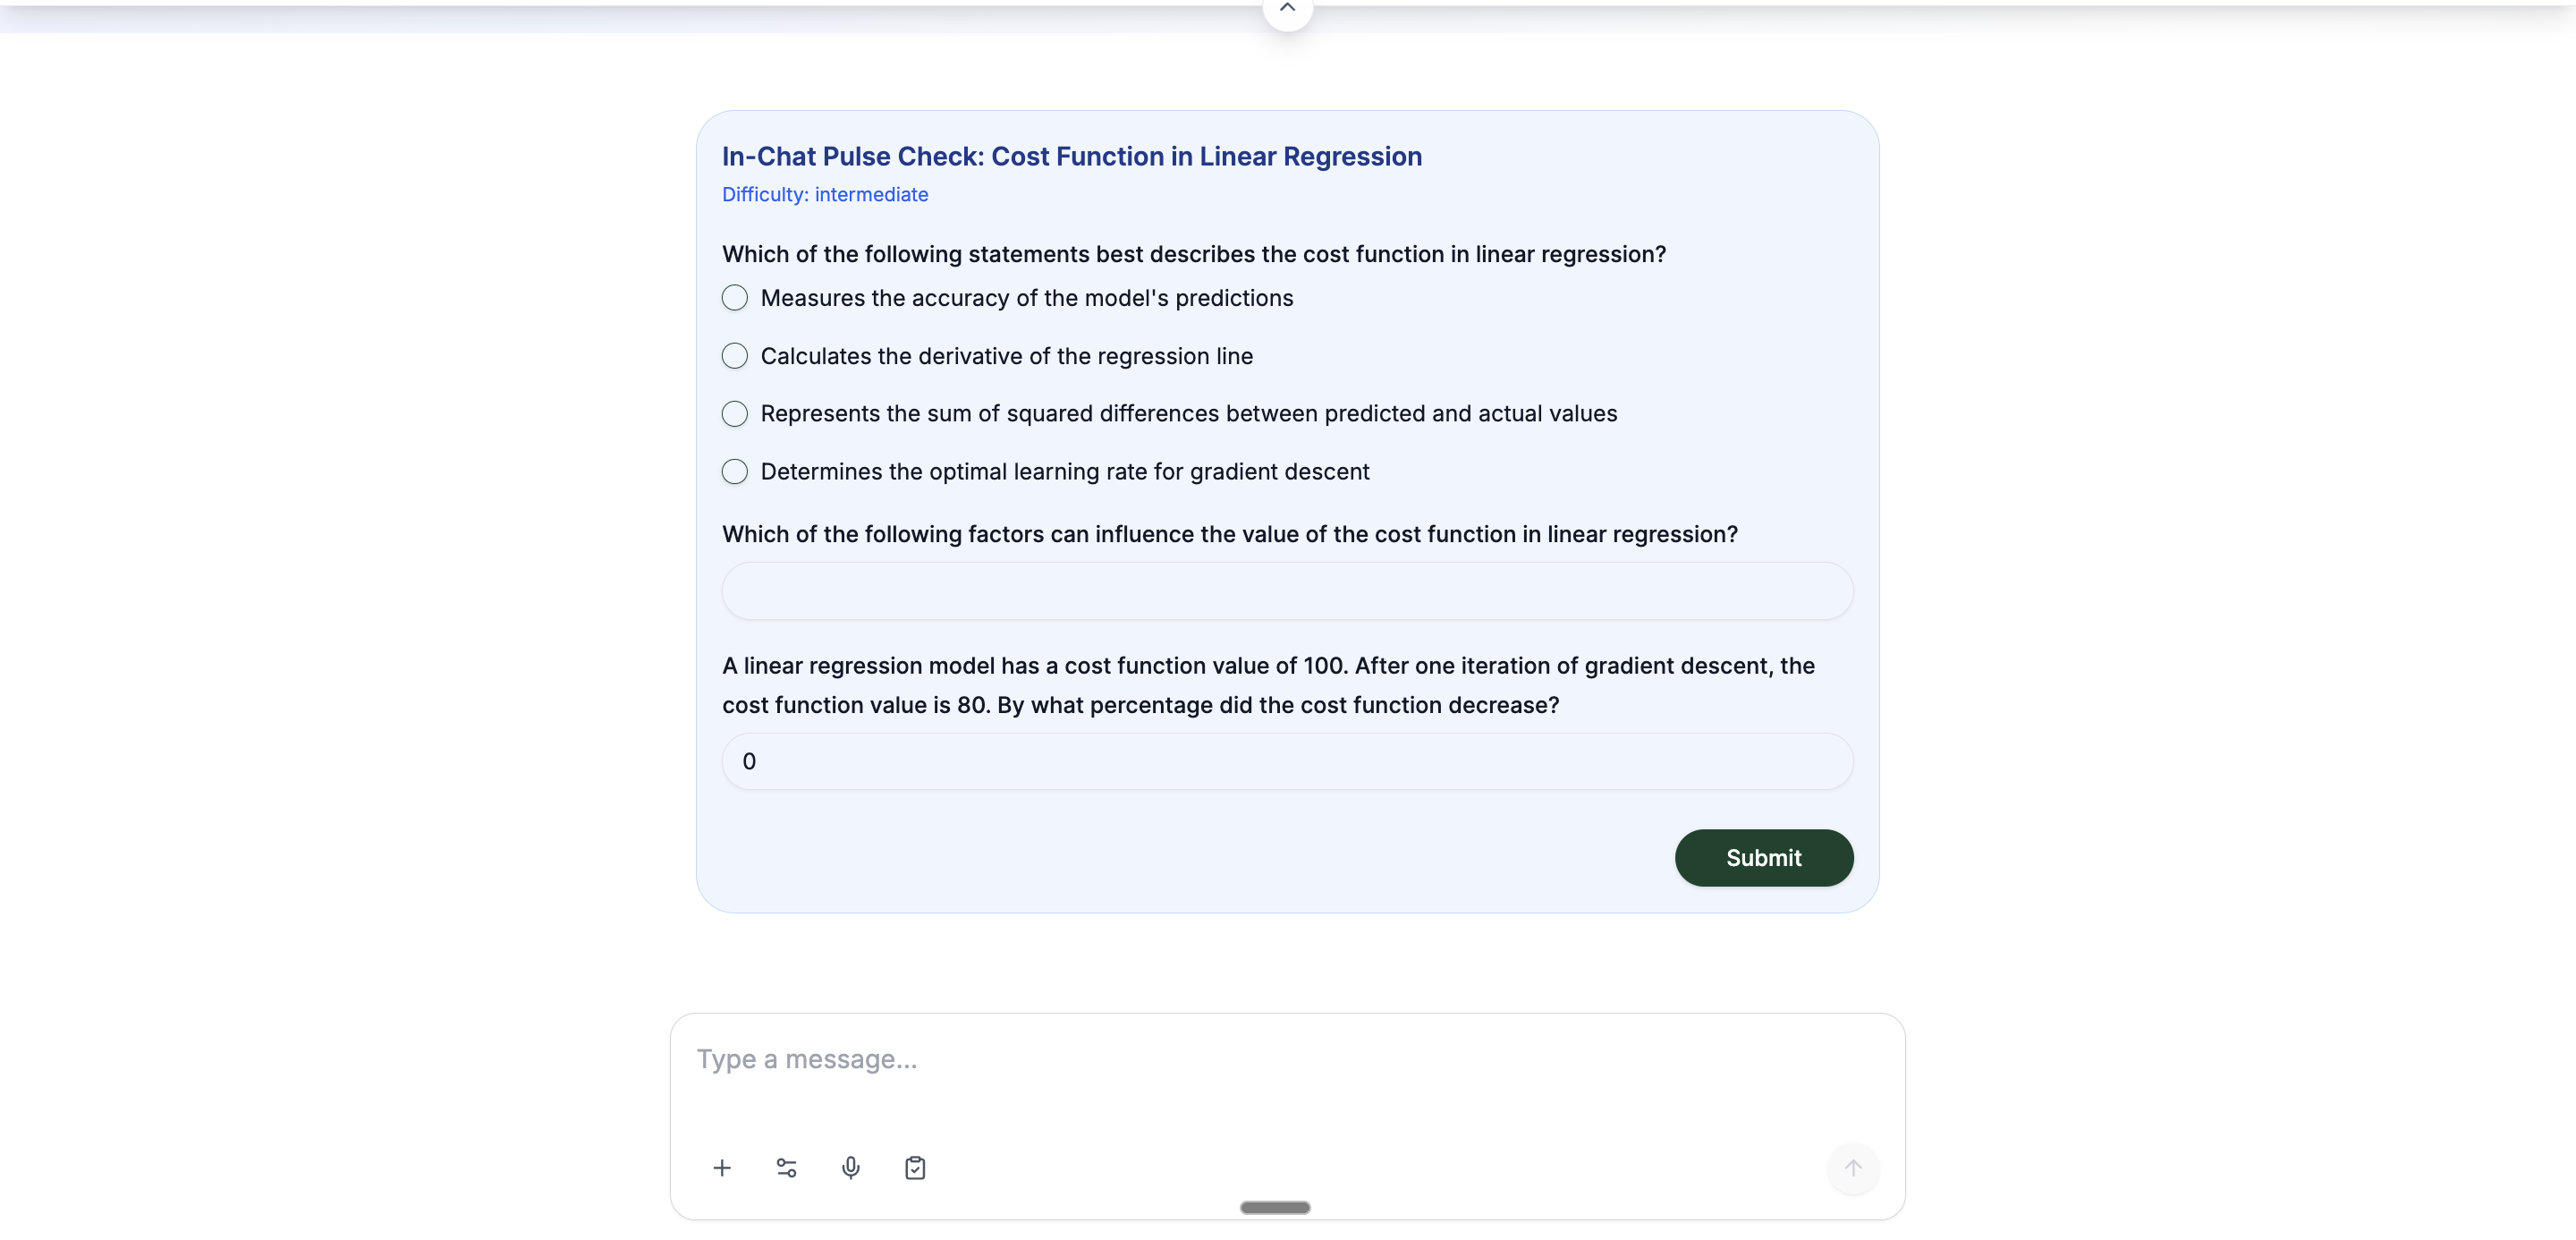
\includegraphics[width=0.8\columnwidth]{figures/adaptive_feedback.png}
\caption{Adaptive feedback interface showing how the system adjusts recommendations based on student performance with transparent explanations.}
\label{fig:adaptive_feedback}
\end{figure}

\subsubsection{System Integration and Data Flow}

The instructor and student workflows are tightly integrated through a shared data infrastructure. Instructor-uploaded materials feed the semantic search system that powers student tutoring interactions. Student survey responses inform pathway generation, which instructors then review and approve. Student performance data aggregates into instructor dashboards without exposing individual identities. This bidirectional flow ensures that personalization remains grounded in instructor-curated content while instructor decisions are informed by student learning patterns.
 
Figure~\ref{fig:overall_system} illustrates how these workflows interconnect through the four core system components: the data ingestion pipeline, survey generation engine, pathway generation module, and intelligent tutoring agent. Each component is designed to maintain the balance between automated personalization and human oversight that emerged as critical during our expert consultation phase.

\subsection{Technical Implementation}

Having established how instructors and students interact with the system, we now detail the technical implementation of each core component that enables these workflows.

\subsection{Component 1: Data Ingestion Pipeline}
\label{sec:data_pipeline}

\subsubsection{Overview and Architecture}

The data ingestion pipeline is responsible for converting instructor-uploaded course materials into a searchable, semantically indexed knowledge base. This component ensures that all student-facing recommendations and tutoring interactions are grounded in actual course content. The pipeline consists of four stages: ingestion and storage, content extraction, chunking and embedding, and vector indexing.

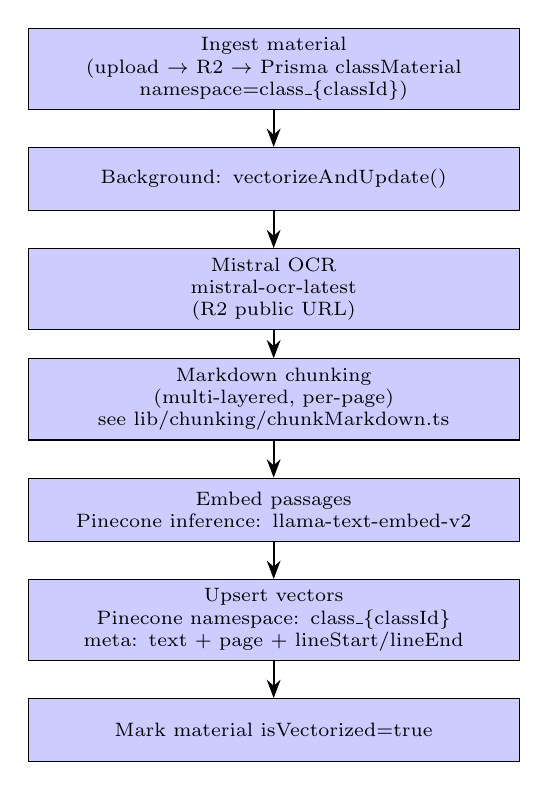
\begin{tikzpicture}[node distance=1.4cm, auto]
    \node (A) [processwide] {Ingest material\\(upload $\rightarrow$ R2 $\rightarrow$ Prisma classMaterial\\namespace=class\_\{classId\})};
    \node (B) [processwide, below of=A] {Background: vectorizeAndUpdate()};
    \node (C) [processwide, below of=B] {Mistral OCR\\mistral-ocr-latest\\(R2 public URL)};
    \node (D) [processwide, below of=C] {Markdown chunking\\(multi-layered, per-page)\\see lib/chunking/chunkMarkdown.ts};
    \node (E) [processwide, below of=D] {Embed passages\\Pinecone inference: llama-text-embed-v2};
    \node (F) [processwide, below of=E] {Upsert vectors\\Pinecone namespace: class\_\{classId\}\\meta: text + page + lineStart/lineEnd};
    \node (G) [processwide, below of=F] {Mark material isVectorized=true};
    
    \draw [arrow] (A) -- (B);
    \draw [arrow] (B) -- (C);
    \draw [arrow] (C) -- (D);
    \draw [arrow] (D) -- (E);
    \draw [arrow] (E) -- (F);
    \draw [arrow] (F) -- (G);
\end{tikzpicture}
\subsubsection{Technical Implementation}

Instructors upload course materials (PDFs, documents, slide presentations) through the platform interface. Materials are immediately stored in Cloudflare R2, a scalable cloud storage service, and registered in the Prisma database with metadata including filename, upload timestamp, and class association. A background vectorization service begins processing asynchronously to avoid blocking the upload flow.

For documents containing visual content (such as slide presentations), we employ Mistral OCR (mistral-ocr-latest) to extract text from images and scanned materials. This Vision Language Model approach preserves the pedagogical intent of visual teaching materials by converting them to queryable text. The extracted text is then combined with any native text content in the document.

Content is chunked using a multi-layered markdown chunking strategy that preserves semantic boundaries. Rather than splitting on fixed token counts, this approach respects section headers, code blocks, and logical divisions within the material. This ensures that related concepts remain grouped and that retrieval results return contextually complete information.

Passages are embedded using Pinecone's inference API with the \texttt{llama-text-embed-v2} model, which creates dense vector representations capturing semantic meaning. Each vector is upserted to a class-specific Pinecone namespace (\texttt{class\_\{classId\}}) with metadata including the original text content, source document name, page number, and line position information. This metadata enables source attribution and allows students to navigate back to original materials.


\subsubsection{Design Rationale}

The decision to use Mistral OCR for visual content processing directly addresses instructor feedback that slide presentations often contain pedagogically important diagrams and visual explanations. By extracting text from visual elements, we ensure that content-heavy slides are searchable without losing fidelity. The use of class-specific namespaces in Pinecone provides data isolation and allows for efficient scaling across multiple courses.

\subsection{Component 2: Survey Generation}

\subsubsection{Overview and Architecture}

The survey generation component creates tailored questionnaires that assess student prerequisite knowledge, learning objectives readiness, assessment preferences, course-specific goals, and learning styles. This information forms the basis for personalized pathway generation. The survey is created by an AI model using course syllabus data and optional instructor context.

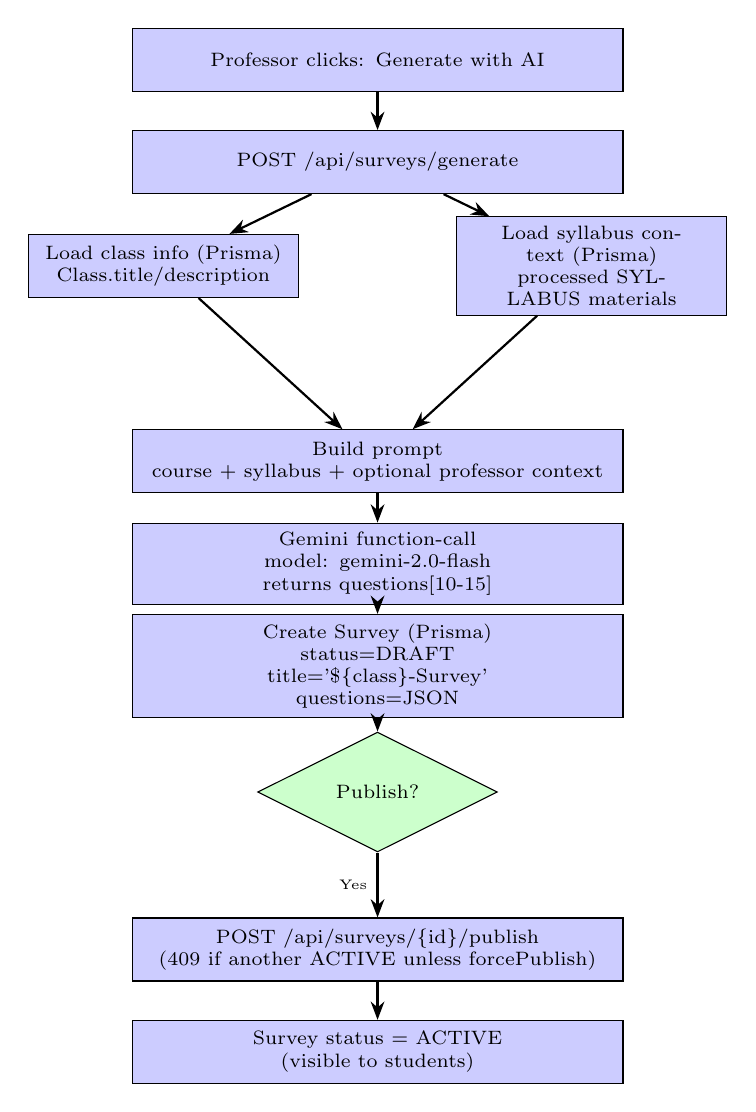
\begin{tikzpicture}[node distance=1.3cm, auto]
    \node (A) [processwide] {Professor clicks: Generate with AI};
    \node (B) [processwide, below of=A] {POST /api/surveys/generate};
    \node (C) [process, below left of=B, xshift=-1.8cm, yshift=-0.4cm] {Load class info (Prisma)\\Class.title/description};
    \node (D) [process, below right of=B, xshift=1.8cm, yshift=-0.4cm] {Load syllabus context (Prisma)\\processed SYLLABUS materials};
    \node (E) [processwide, below of=B, yshift=-2.5cm] {Build prompt\\course + syllabus + optional professor context};
    \node (F) [processwide, below of=E] {Gemini function-call\\model: gemini-2.0-flash\\returns questions[10-15]};
    \node (G) [processwide, below of=F] {Create Survey (Prisma)\\status=DRAFT\\title='\$\{class\}-Survey'\\questions=JSON};
    \node (H) [decision, below of=G, yshift=-0.3cm] {Publish?};
    \node (I) [processwide, below of=H, yshift=-0.7cm] {POST /api/surveys/\{id\}/publish\\(409 if another ACTIVE unless forcePublish)};
    \node (J) [processwide, below of=I] {Survey status = ACTIVE\\(visible to students)};
    
    \draw [arrow] (A) -- (B);
    \draw [arrow] (B) -- (C);
    \draw [arrow] (B) -- (D);
    \draw [arrow] (C) -- (E);
    \draw [arrow] (D) -- (E);
    \draw [arrow] (E) -- (F);
    \draw [arrow] (F) -- (G);
    \draw [arrow] (G) -- (H);
    \draw [arrow] (H) -- node[anchor=east, font=\tiny] {Yes} (I);
    \draw [arrow] (I) -- (J);
\end{tikzpicture}

\subsubsection{Technical Implementation}

When an instructor initiates survey generation, the system retrieves course information (title, description, learning objectives, prerequisites, assessment methods) from the syllabus database along with any previously uploaded course materials. The instructor may optionally provide additional context or emphasis areas.

The system constructs a detailed prompt that includes all available course information and passes this to Gemini 2.0 Flash configured for function calling. The model generates 10--15 survey questions organized into five categories: prerequisite assessment, learning objectives readiness, assessment preparation, course-specific goals, and learning preferences and challenges.

\definecolor{customcolor}{HTML}{E7DCE4}
\begin{tcolorbox}[breakable, colframe=customcolor, colback=customcolor!30!white, coltitle=black, title=Survey Generation Prompt, fontupper=\small]
\textbf{You are an expert educational assessment specialist.} Generate a comprehensive student survey for personalized learning path creation based on the following course information:

\vspace{0.5em}
\textbf{COURSE DETAILS:}
\begin{itemize}
    \item Course Name, Description, Academic Level
    \item Prerequisites, Learning Objectives
    \item Assessment Methods, Course Schedule, Grading Policy
\end{itemize}

\vspace{0.5em}
Generate 10--15 survey questions that are specifically tailored to this course. Focus on:

\begin{enumerate}
    \item \textbf{Prerequisite Assessment:} Assessing specific knowledge areas mentioned in prerequisites
    \item \textbf{Learning Objectives Readiness:} Assessing readiness for specific learning outcomes
    \item \textbf{Assessment Preparation:} Understanding student preferences for evaluation methods
    \item \textbf{Course-Specific Goals:} Understanding student goals aligned with course content
    \item \textbf{Learning Preferences \& Challenges:} Identifying learning style and preferences
\end{enumerate}

\vspace{0.5em}
\textbf{IMPORTANT REQUIREMENTS:} Make questions SPECIFIC to this course's actual content and use clear, student-friendly language.
\end{tcolorbox}

% \textit{Survey Generation Prompt:}
% \begin{quote}
% \small\itshape
% You are an expert educational assessment specialist. Generate a comprehensive student survey for personalized learning path creation based on the following course information:

% COURSE DETAILS:
% - Course Name, Description, Academic Level
% - Prerequisites, Learning Objectives
% - Assessment Methods, Course Schedule, Grading Policy

% Generate 10--15 survey questions that are specifically tailored to this course. Focus on: (1)~PREREQUISITE ASSESSMENT assessing specific knowledge areas mentioned in prerequisites; (2)~LEARNING OBJECTIVES READINESS assessing readiness for specific learning outcomes; (3)~ASSESSMENT PREPARATION understanding student preferences for evaluation methods; (4)~COURSE-SPECIFIC GOALS understanding student goals aligned with course content; (5)~LEARNING PREFERENCES \& CHALLENGES identifying learning style and preferences.

% IMPORTANT REQUIREMENTS: Make questions SPECIFIC to this course's actual content and use clear, student-friendly language.
% \end{quote}

Generated questions are stored as a draft survey in the database. Instructors review the draft, make edits if needed, and then publish the survey. Once published, the survey becomes visible to students at the start of the course. The system prevents multiple active surveys in the same class unless explicitly overridden.

\subsubsection{Design Rationale}

The structured categories in the survey prompt ensure that the AI generates questions aligned with pedagogically relevant dimensions. By grounding survey generation in actual course syllabi rather than generic templates, we ensure that questions are specific and actionable. The draft-review-publish workflow maintains instructor oversight, addressing stakeholder feedback that instructors must retain control over student-facing content.

\subsection{Component 3: Pathway Generation}

\subsubsection{Overview and Architecture}

The pathway generation component creates a personalized sequence of learning nodes tailored to each student's survey responses and learning context. Each node represents a focused learning objective, complete with recommended resources, prerequisite information, and assessment opportunities. The pathway is structured to respect cognitive progression and align with course learning objectives.

\begin{figure}[h]
\centering
\resizebox{0.5\textwidth}{!}{%
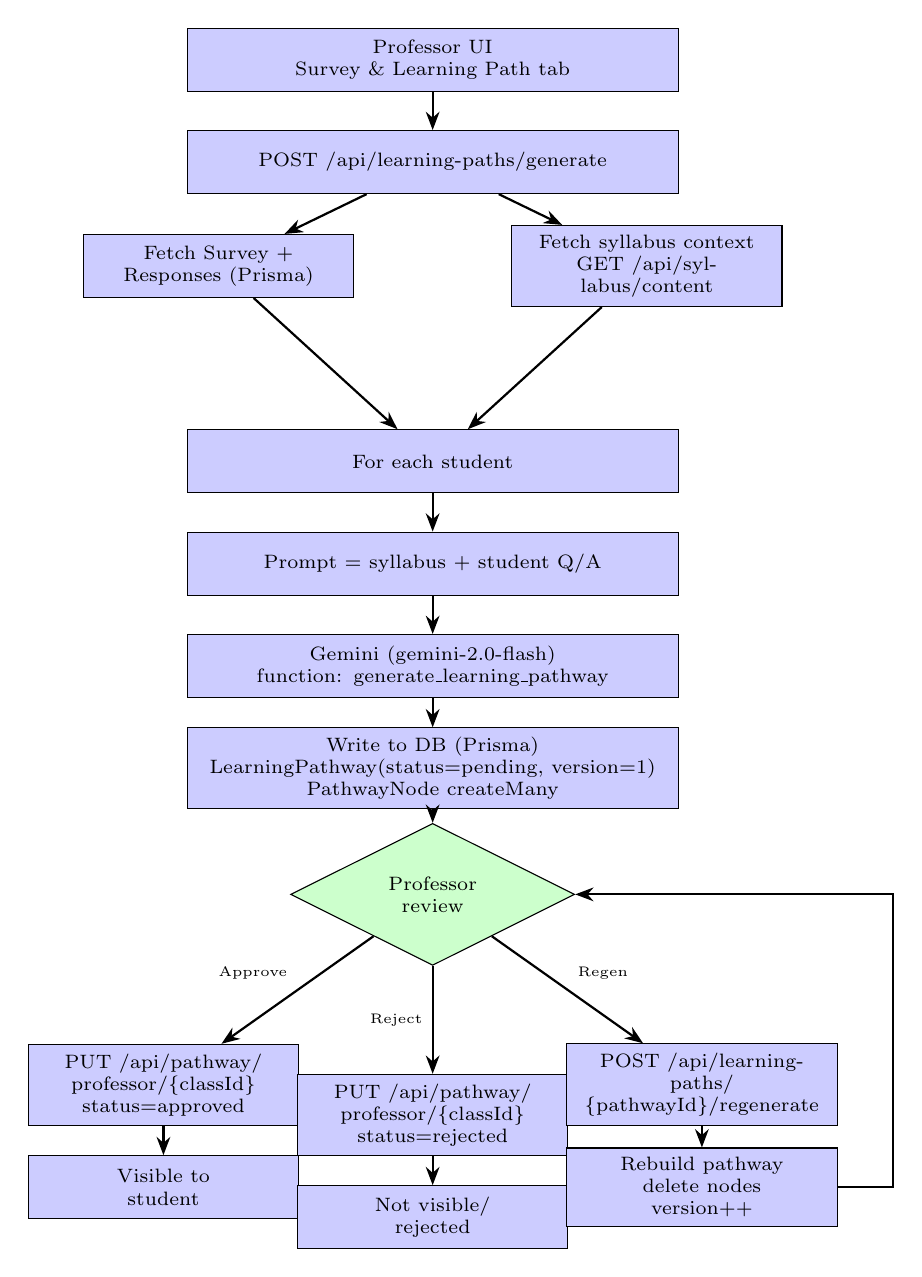
\begin{tikzpicture}[node distance=1.3cm, auto]
    \node (A) [processwide] {Professor UI\\Survey \& Learning Path tab};
    \node (B) [processwide, below of=A] {POST /api/learning-paths/generate};
    \node (C) [process, below left of=B, xshift=-1.8cm, yshift=-0.4cm] {Fetch Survey +\\Responses (Prisma)};
    \node (D) [process, below right of=B, xshift=1.8cm, yshift=-0.4cm] {Fetch syllabus context\\GET /api/syllabus/content};
    \node (E) [processwide, below of=B, yshift=-2.5cm] {For each student};
    \node (F) [processwide, below of=E] {Prompt = syllabus + student Q/A};
    \node (G) [processwide, below of=F] {Gemini (gemini-2.0-flash)\\function: generate\_learning\_pathway};
    \node (H) [processwide, below of=G] {Write to DB (Prisma)\\LearningPathway(status=pending, version=1)\\PathwayNode createMany};
    \node (R) [decision, below of=H, yshift=-0.3cm] {Professor\\review};
    \node (P) [process, below left of=R, xshift=-2.5cm, yshift=-1.5cm] {PUT /api/pathway/\\professor/\{classId\}\\status=approved};
    \node (Q) [process, below of=R, yshift=-1.5cm] {PUT /api/pathway/\\professor/\{classId\}\\status=rejected};
    \node (S) [process, below right of=R, xshift=2.5cm, yshift=-1.5cm] {POST /api/learning-paths/\\\{pathwayId\}/regenerate};
    \node (P2) [process, below of=P] {Visible to\\student};
    \node (Q2) [process, below of=Q] {Not visible/\\rejected};
    \node (S2) [process, below of=S] {Rebuild pathway\\delete nodes\\version++};
    
    \draw [arrow] (A) -- (B);
    \draw [arrow] (B) -- (C);
    \draw [arrow] (B) -- (D);
    \draw [arrow] (C) -- (E);
    \draw [arrow] (D) -- (E);
    \draw [arrow] (E) -- (F);
    \draw [arrow] (F) -- (G);
    \draw [arrow] (G) -- (H);
    \draw [arrow] (H) -- (R);
    \draw [arrow] (R) -- node[anchor=south east, font=\tiny] {Approve} (P);
    \draw [arrow] (R) -- node[anchor=east, font=\tiny] {Reject} (Q);
    \draw [arrow] (R) -- node[anchor=south west, font=\tiny] {Regen} (S);
    \draw [arrow] (P) -- (P2);
    \draw [arrow] (Q) -- (Q2);
    \draw [arrow] (S) -- (S2);
    \draw [arrow] (S2.east) -- ++(0.7,0) |- (R.east);
\end{tikzpicture}
}

\end{figure}

\subsubsection{Technical Implementation}

Once students complete the initial survey, instructors trigger pathway generation through the platform. The system fetches the student's survey responses and the course syllabus context from the database. It then constructs a detailed prompt that combines course information, student answers, and pedagogical guidelines.

Gemini 2.0 Flash, configured for function calling, generates a structured learning pathway specifying 10--14 pathway nodes. Each node includes a title, description, learning objectives, recommended content from the class materials (with source attribution), sequencing information, and alignment with Bloom's taxonomy levels. The pathway generation respects prerequisite relationships and adapts sequencing based on the student's prior knowledge as indicated in survey responses.

\definecolor{customcolor}{HTML}{E7DCE4}
\begin{tcolorbox}[breakable, colframe=customcolor, colback=customcolor!30!white, coltitle=black, title=Pathway Generation Prompt, fontupper=\small]
\textbf{Course Information:}
\begin{itemize}
    \item Description, Prerequisites, Learning Objectives
    \item Course Schedule, Assessment Methods
\end{itemize}

\vspace{0.5em}
\textbf{Student Survey Responses:} [Student answers mapped to survey questions]

\vspace{0.5em}
Based on the course information and the student's survey responses, generate a personalized learning pathway that:

\begin{enumerate}
    \item Aligns with the course learning objectives and schedule
    \item Considers the student's learning preferences, prior knowledge, and interests
    \item Takes into account any prerequisites or background knowledge gaps
    \item Incorporates the assessment methods and grading structure
    \item Provides a structured progression through the course material with clear dependencies
\end{enumerate}

\vspace{0.5em}
\textbf{Output:} Create 10--14 pathway nodes that form a coherent learning journey.

\end{tcolorbox}

% \textit{Pathway Generation Prompt:}
% \begin{quote}
% \small\itshape{Course Information: Description, Prerequisites, Learning Objectives, Course Schedule, Assessment Methods

% Student Survey Responses: [Student answers mapped to survey questions]

% Based on the course information and the student's survey responses, generate a personalized learning pathway that: (1) Aligns with the course learning objectives and schedule; (2) Considers the student's learning preferences, prior knowledge, and interests; (3) Takes into account any prerequisites or background knowledge gaps; (4) Incorporates the assessment methods and grading structure; (5) Provides a structured progression through the course material with clear dependencies.

% Create 10-14 pathway nodes that form a coherent learning journey.
% \end{quote}

The generated pathway is stored in the database as a pending version with all nodes. Instructors review the pathway through a structured review interface and can take three actions: approve it to make it visible to the student, reject it with feedback, or regenerate it with additional focus areas. The regeneration workflow increments the pathway version, clears previous nodes, and regenerates the pathway with updated constraints, maintaining a full audit trail of all versions.

\subsubsection{Design Rationale}

The pathway generation prompt explicitly includes syllabus information, course schedule, and assessment methods to ensure that generated pathways respect the actual course structure and pacing. By embedding student survey responses directly in the prompt, the model tailors the pathway to individual needs rather than creating generic sequences. The approval-rejection-regeneration workflow addresses stakeholder feedback about instructor control and allows iterative refinement if the initial pathway does not match pedagogical expectations.

\subsection{Component 4: Intelligent Tutoring Agent}

\subsubsection{Overview and Architecture}

The intelligent tutoring agent provides one-on-one tutoring support as students engage with their personalized pathways. The agent uses the Socratic method to guide learning, dynamically retrieves relevant class materials using RAG, and can generate formative assessments to check understanding. All interactions are grounded in instructor-provided content.
\begin{figure}[h]
\centering
\resizebox{0.5\textwidth}{!}{%
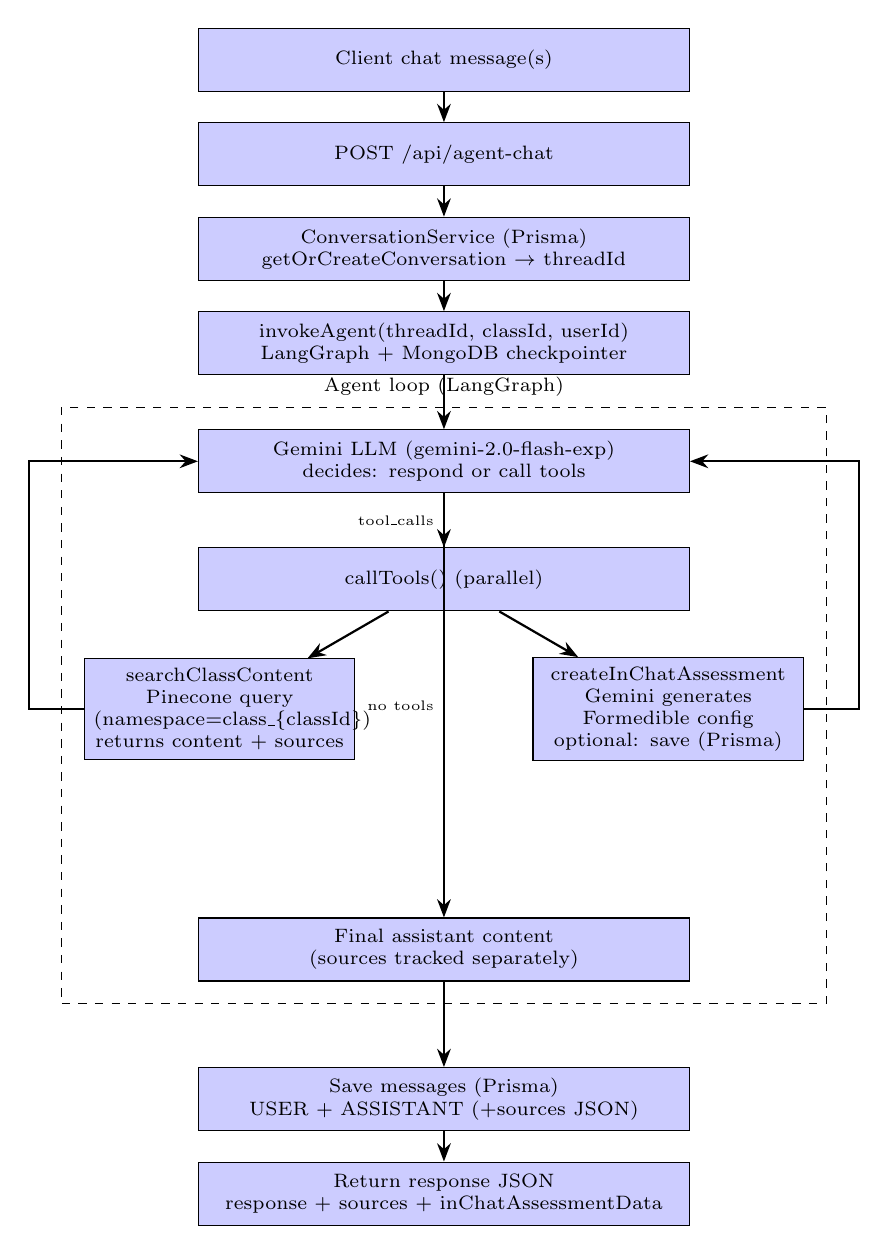
\begin{tikzpicture}[node distance=1.2cm, auto]
    \node (A) [processwide] {Client chat message(s)};
    \node (B) [processwide, below of=A] {POST /api/agent-chat};
    \node (C) [processwide, below of=B] {ConversationService (Prisma)\\getOrCreateConversation $\rightarrow$ threadId};
    \node (D) [processwide, below of=C] {invokeAgent(threadId, classId, userId)\\LangGraph + MongoDB checkpointer};
    
    % Subgraph for Agent loop
    \node (E) [processwide, below of=D, yshift=-0.3cm] {Gemini LLM (gemini-2.0-flash-exp)\\decides: respond or call tools};
    \node (F) [processwide, below of=E, yshift=-0.3cm] {callTools() (parallel)};
    \node (F1) [process, below left of=F, xshift=-2cm, yshift=-0.8cm] {searchClassContent\\Pinecone query\\(namespace=class\_\{classId\})\\returns content + sources};
    \node (F2) [process, below right of=F, xshift=2cm, yshift=-0.8cm] {createInChatAssessment\\Gemini generates\\Formedible config\\optional: save (Prisma)};
    \node (H) [processwide, below of=F, yshift=-3.5cm] {Final assistant content\\(sources tracked separately)};
    
    \begin{scope}[on background layer]
        \node[subgraph, fit=(E)(F)(F1)(F2)(H), label=above:\scriptsize Agent loop (LangGraph)] (subG) {};
    \end{scope}
    
    \node (I) [processwide, below of=H, yshift=-0.7cm] {Save messages (Prisma)\\USER + ASSISTANT (+sources JSON)};
    \node (J) [processwide, below of=I] {Return response JSON\\response + sources + inChatAssessmentData};
    
    \draw [arrow] (A) -- (B);
    \draw [arrow] (B) -- (C);
    \draw [arrow] (C) -- (D);
    \draw [arrow] (D) -- (E);
    \draw [arrow] (E) -- node[anchor=east, font=\tiny] {tool\_calls} (F);
    \draw [arrow] (F) -- (F1);
    \draw [arrow] (F) -- (F2);
    \draw [arrow] (F1.west) -- ++(-0.7,0) |- (E.west);
    \draw [arrow] (F2.east) -- ++(0.7,0) |- (E.east);
    \draw [arrow] (E) -- node[anchor=east, font=\tiny] {no tools} (H);
    \draw [arrow] (H) -- (I);
    \draw [arrow] (I) -- (J);
\end{tikzpicture}
}
\end{figure}

\subsubsection{Technical Implementation}

Students interact with their learning pathways through a chat interface. When a student sends a message, the request is processed by a LangGraph-based agent running on a MongoDB checkpointer for stateful conversation management. The agent decides whether to respond directly or invoke tools based on the message content and context.

The \texttt{searchClassContent} tool enables the agent to query Pinecone for relevant class materials. When called, it performs a semantic search within the class-specific namespace and returns passages with full source attribution. This ensures that all content-specific responses are grounded in actual course materials.

The \texttt{createInChatAssessment} tool generates formative assessments using Gemini. When invoked, it accepts parameters including the topic, node title (if available), question count, and difficulty level. The model generates a quiz configured in Formedible format, and instructors can optionally save these assessments to the database for later review and analytics.

All conversations are logged in Prisma, including user messages, assistant responses, tool invocations, and sources. This enables instructors to understand student learning patterns and identify concepts where many students struggle.

\subsubsection{Agent System Prompt and Socratic Method}

The agent operates under a detailed system prompt that establishes its educational role and decision-making priorities:

\definecolor{customcolor}{HTML}{E7DCE4}
\begin{tcolorbox}[breakable, colframe=customcolor, colback=customcolor!30!white, coltitle=black, title=Agent System Prompt, fontupper=\small]
\small{You are a highly capable educational assistant for Synapsed, designed to help students learn effectively.

CORE DIRECTIVES:

1. GROUNDING \& TOOL USAGE: When asked about class-specific concepts, YOU MUST use the searchClassContent tool to ensure accuracy. For greetings or general advice, you may answer directly without tools. Do NOT include source citations in your response---sources are tracked automatically by the system.

2. TEACHING STYLE (SOCRATIC): DO NOT simply give answers to homework or complex conceptual questions. GUIDE the student by asking probing questions to help them arrive at the answer themselves. Break down complex topics into smaller, digestible steps.

3. ADAPTABILITY: Tailor your explanations to the student's level. Use analogies and examples to clarify difficult concepts.

4. IN-CHAT ASSESSMENT: After explaining a concept or topic, assess the student's understanding by using the createInChatAssessment tool. Provide constructive feedback on their answers, highlighting what they understood well and areas for improvement. Continue the conversation naturally, addressing any gaps in understanding.}
\end{tcolorbox}

% \textit{Agent System Prompt:}
% \begin{quote}
% \small\itshape{You are a highly capable educational assistant for Synapsed, designed to help students learn effectively.

% CORE DIRECTIVES:

% 1. GROUNDING \& TOOL USAGE: When asked about class-specific concepts, YOU MUST use the searchClassContent tool to ensure accuracy. For greetings or general advice, you may answer directly without tools. Do NOT include source citations in your response---sources are tracked automatically by the system.

% 2. TEACHING STYLE (SOCRATIC): DO NOT simply give answers to homework or complex conceptual questions. GUIDE the student by asking probing questions to help them arrive at the answer themselves. Break down complex topics into smaller, digestible steps.

% 3. ADAPTABILITY: Tailor your explanations to the student's level. Use analogies and examples to clarify difficult concepts.

% 4. IN-CHAT ASSESSMENT: After explaining a concept or topic, assess the student's understanding by using the createInChatAssessment tool. Provide constructive feedback on their answers, highlighting what they understood well and areas for improvement. Continue the conversation naturally, addressing any gaps in understanding.}
% \end{quote}

\subsubsection{Node Introduction Prompt}

When a student begins a new learning pathway node, they are greeted with an engaging introduction that uses the Socratic method. The introduction prompt directs the agent to first retrieve relevant materials using RAG:
\definecolor{customcolor}{HTML}{E7DCE4}
\begin{tcolorbox}[breakable, colframe=customcolor, colback=customcolor!30!white, coltitle=black, title=Node Introduction Prompt, fontupper=\small]
You are an AI tutor using the Socratic teaching method. A student is starting to learn about ``[nodeTitle]''.

\vspace{0.5em}
\textbf{CRITICAL FIRST STEP:} Before introducing the topic, you MUST use the \texttt{searchClassContent} tool to retrieve relevant information about ``[nodeTitle]'' from the class materials. This ensures you have accurate, up-to-date information about what this topic covers in this specific class.

\vspace{0.5em}
\textbf{After retrieving the information:}

\begin{enumerate} 
    \item Use the retrieved content to introduce [nodeTitle] with an engaging, thought-provoking question that connects to their prior knowledge
    \item Reference specific information from the class materials when relevant
    \item Use questions to guide their learning rather than lecturing---help them discover concepts through dialogue
    \item Build on their responses with follow-up questions that encourage critical thinking
    \item Make the conversation interactive and conversational
\end{enumerate}

\vspace{0.5em}
\textbf{IMPORTANT:} You MUST call \texttt{searchClassContent} FIRST before responding. Do not skip this step.

\end{tcolorbox}

% \textit{Node Introduction Prompt:}
% \begin{quote}
% \small\itshape{You are an AI tutor using the Socratic teaching method. A student is starting to learn about ``[nodeTitle]''.

% CRITICAL FIRST STEP: Before introducing the topic, you MUST use the searchClassContent tool to retrieve relevant information about ``[nodeTitle]'' from the class materials. This ensures you have accurate, up-to-date information about what this topic covers in this specific class.

% After retrieving the information:
% 1. Use the retrieved content to introduce [nodeTitle] with an engaging, thought-provoking question that connects to their prior knowledge
% 2. Reference specific information from the class materials when relevant
% 3. Use questions to guide their learning rather than lecturing---help them discover concepts through dialogue
% 4. Build on their responses with follow-up questions that encourage critical thinking
% 5. Make the conversation interactive and conversational

% IMPORTANT: You MUST call searchClassContent FIRST before responding. Do not skip this step.
% \end{quote}

This prompt ensures that every node introduction is grounded in the actual course materials and uses pedagogically sound Socratic questioning rather than lecturing.

\subsubsection{Design Rationale}

The agent architecture separates concerns: the LLM handles dialogue and reasoning, tools handle content retrieval and assessment generation, and the database handles logging and state persistence. This modular design allows each component to be refined independently.

The Socratic method is enforced through the system prompt rather than trusted to emerge naturally, and this choice has empirical backing. Liu et al.~\cite{liu2024socraticlm} demonstrate that current LLMs, including GPT-4, ``predominantly follow a Question-Answering paradigm'' and give direct answers even when explicitly instructed to teach Socratically. Bonino et al.~\cite{bonino2024euler} confirm the same failure in a qualitative analysis: GPT-4 states the answer directly in their sample output, which they note ``contradicts the demands of Socratic teaching.'' MathTutorBench~\cite{macina2025mathtutorbench} finds that ``subject expertise does not immediately translate to good teaching'' and that ``tutoring becomes more challenging in longer dialogs, where simpler questioning strategies begin to fail.'' These findings are why SynapsEd's system prompt explicitly prohibits direct answers and requires the agent to guide students through questions, rather than simply instructing it to ``be a good tutor'' and hoping for the best.

The explicit grounding in class-specific tools (searchClassContent) ensures accuracy and maintains instructor oversight by keeping all responses within the curriculum. The SocraticRAG benchmark paper being developed in parallel will provide the evaluation infrastructure to measure how well SynapsEd's agent actually performs on these dimensions in future work.

\section{Semester 2 Feature Extensions}
\label{sec:s2features}

\subsection{Feature 1: Voice-Based Learning}

\subsubsection{Overview}

The voice-based learning feature enables bidirectional spoken interaction between students and the AI tutor. Students speak their questions or responses; the system converts speech to text, processes it through the tutoring agent, and delivers the AI's reply as synthesized speech. This transforms the SynapsEd tutoring interface from a text chat into an interactive multimodal learning environment in which ``the learner can ask a question and receive an answer, or can give an answer and receive feedback''~\cite{moreno2007interactive}.

\subsubsection{Design Rationale}

When a student is reading an AI tutoring response as text, they are doing two visual tasks at once: parsing the explanation and looking at the pathway, source attributions, and any diagrams on screen. Both tasks compete for the same visual channel, and when they overlap, neither gets full attention. The solution Moreno and Mayer~\cite{moreno2007interactive} established is to split the load: present verbal content through the auditory modality and keep the visual channel free for non-verbal material. ``The most effective learning environments,'' they write, ``are those that combine verbal and non-verbal representations of the knowledge using mixed-modality presentations.'' Mayer~\cite{mayer2021instructional} confirms the magnitude of the effect, with narrated animation outperforming text-only narration by $d = 1.90$ on transfer tests. The voice feature applies this directly: the AI's response comes through the speaker, the student's eyes stay on the course content.

What makes voice more than a delivery preference is that spoken dialogue is itself a learning mechanism. Moreno and Mayer define ``dialoguing interactivity'' as the mode in which ``the learner can ask a question and receive an answer, or can give an answer and receive feedback''~\cite{moreno2007interactive}: this is exactly what happens when a student speaks to the tutor and the tutor speaks back. Fiorella and Mayer~\cite{fiorella2016generative} show that strategies activating this kind of verbal interaction, including imagining and self-explaining, trigger the same process that makes learning durable: actively reorganizing new information and connecting it to what the student already knows.

\subsubsection{Implementation}

The feature uses text-to-speech and speech-to-text APIs integrated into the SynapsEd chat interface. The tutoring agent pipeline is unchanged: speech input is transcribed and passed to the LangGraph agent, which retrieves relevant class materials and generates a response. The response text is then converted to speech and played back to the student. All interactions are logged identically to text sessions, preserving source attribution and conversation history.

\subsection{Feature 2: Drawing-Based Visual Explanation}

\subsubsection{Overview}

The drawing-based visual explanation feature enables the AI tutor to generate Excalidraw~\cite{excalidraw2024} diagrams as part of its tutoring responses. When the AI determines that a visual explanation would support understanding, it produces a structured diagram alongside its text response. The diagram renders directly in the chat interface.

\subsubsection{Design Rationale}

Visual representations work because they make abstract ideas concrete. Rau~\cite{rau2017visual} reviews the evidence across STEM learning and finds that ``visual representations can help students learn because they make abstract concepts accessible,'' with effects strongest for students with low prior knowledge. Fiorella and Mayer~\cite{fiorella2016generative} show that creating a drawing is itself a learning mechanism: it forces the student to select the relevant information, organize it spatially, and connect it to what they already know. The drawing group outperformed controls by $d = 0.81$, and the effect was largest for spatial and abstract material.

The problem is that drawing is cognitively expensive. Students who are still learning a concept cannot easily depict it; the effort of figuring out what to draw competes with the effort of understanding the concept. Rau~\cite{rau2017visual} calls this the representation dilemma: how do you learn from a representation you do not yet understand, while simultaneously learning the content it is supposed to show? SynapsEd resolves this by generating the diagram for the student. The AI produces the Excalidraw structure and the student reads and explores it. The generative benefit, integrating visual and verbal information into a coherent mental model, is preserved without the mechanical burden.

Diagrams are not shown for every concept. The feature is triggered when the concept is spatial or abstract, or when the student's onboarding survey indicated a preference for visual explanations. This follows Walkington and Bernacki~\cite{walkington2019personalizing}, who find that personalizing ITS content to student-expressed preferences improves engagement and reduces off-task behavior. The visual modality is available to all students; what changes is which presentation is surfaced first, not which is withheld.

\subsubsection{Implementation}

When the tutoring agent decides to generate a diagram, it constructs an Excalidraw JSON specification describing the diagram elements (shapes, labels, arrows) and passes it to a rendering component embedded in the chat interface. The specification is generated by the same Gemini model that produces the text response, in a structured function-calling format. The resulting diagram renders as an interactive Excalidraw canvas inside the chat, which the student can zoom and explore. The AI's text explanation accompanies the diagram, so verbal and visual representations are always presented together~\cite{rau2017visual}.

\subsection{Feature 3: Mastery-Gated Quizzes}

\subsubsection{Overview}

The mastery-gated quiz system requires students to demonstrate understanding through 2--3 in-chat assessments before the formal quiz section for a learning node unlocks. Students who score below a threshold receive targeted feedback and may reattempt. Students who pass unlock the formal assessment. The goal is to confirm learning before summative evaluation, rather than allowing students to advance without engagement.

\subsubsection{Design Rationale}

Bloom's 2 sigma study~\cite{bloom1984sigma} is one of the most cited findings in educational research: students who receive mastery-based instruction, where they must demonstrate understanding before advancing, score approximately one standard deviation above conventional class averages. About 70\% of mastery learners reach the achievement level of only the top 20\% under conventional instruction. The finding holds across subjects and age groups, and the mechanism is straightforward: students advance when they understand the material, not when the scheduled time is up.

The mastery gate applies this principle inside SynapsEd's existing infrastructure. The in-chat assessments that the tutoring agent already generates become a prerequisite rather than optional practice. A student who performs well unlocks the formal quiz for that node; a student who does not returns to the tutoring conversation and engages with the concept further before trying again. The DKT component from Semester 1 tracks performance across nodes and informs the gate threshold. This makes mastery-based progression a natural extension of the system's existing feedback loop rather than a bolted-on restriction.

There is also a behavioral dimension. Students who participated in the Semester 1 consultation raised the concern that a system they can click through quickly might push them toward external AI shortcuts instead of genuine engagement. Walkington and Bernacki~\cite{walkington2019personalizing} found that ITS personalization to student profile ``reduces gaming the system.'' The mastery gate addresses the same problem from a structural angle: if demonstrating understanding is the only way to unlock the next stage, the shortcut value of passive navigation disappears.

\subsubsection{Implementation}

The mastery gate is built on top of the DKT component from Semester 1, which already tracks student performance across learning nodes. The in-chat assessment tool (\texttt{createInChatAssessment}) from the tutoring agent generates the pre-gate quizzes. Once a student's DKT-estimated mastery for a node exceeds a configurable threshold, the formal quiz section for that node is unlocked and visible in the pathway interface. The mastery threshold is a design parameter currently under calibration; empirical validation is planned for the longitudinal study.

\textbf{Status:} This feature is currently under development. The formal quiz unlock mechanism and mastery threshold calibration are not yet empirically validated in SynapsEd. Claims about its effectiveness are based on the mastery learning literature~\cite{bloom1984sigma} and represent design hypotheses to be tested in the planned longitudinal study.

\section{Expert Consultation and Design Refinement}
\label{sec:expert}

Semester 1 included structured expert consultation to validate and refine system design. Findings directly informed the architecture of all four core system components.

\subsection{Instructor Consultation (n=8)}

We conducted 8 semi-structured interviews~\cite{ruslin2022semistructured} with educational specialists from HB CLT staff and NYUAD Head of Programs. Interviews focused on system feasibility, pedagogical soundness, and integration into teaching practice.

\textbf{Key Findings:}

\textit{Prerequisite Mapping as a Core Priority:} Faculty emphasized that fine-grained prerequisite mapping was highly valuable. Rather than requiring students to complete entire prerequisite courses, the system could focus learners on the 10\% of foundational knowledge actually needed for a topic. This addresses both efficiency and learner motivation.

\textit{Instructor Control and Fairness:} Multiple instructors highlighted that personalization must support deficiency-based guidance (addressing gaps) while ensuring all students have access to the same underlying resources. This prevents the appearance of unfair or opaque differentiation and maintains transparency about what content is available to whom.

\textit{Workload Reduction:} Faculty identified automation of semester assessment reports and course archives as a critical feature that would improve adoption. Manual reporting is currently time-intensive.

\textit{Feedback and Content Improvement:} Instructors requested mechanisms to surface which concepts students struggle with or search for externally, enabling instructors to refine their own materials based on learner needs.

These findings directly shaped our system design, prioritizing explicit prerequisite relationships, transparent content allocation, and data aggregation for instructor reflection.

\subsection{Student Consultation (n=6)}

We conducted 6 semi-structured interviews with potential student end-users to gather usability and engagement feedback on early interface prototypes.

\textbf{Key Findings:}

\textit{Clarity and Navigation:} Students emphasized the importance of clear labeling, intuitive layout, and straightforward instructions. Students preferred minimalist interfaces that did not overwhelm with options.

\textit{Engagement and Motivation:} Students saw value in the system as a teaching assistant rather than a burden. Features that reduce friction (e.g., synthesizing materials rather than requiring navigation across many sources) were viewed positively.

\textit{Pathway Representation:} Visual design of learning journeys was important. Students wanted to understand their progress and see the relationship between nodes.

\textit{Transparency:} Students were willing to trust AI recommendations if explanations were clear. Vague or unexplained suggestions would reduce engagement.

\textit{Avoiding Misuse:} Students raised concerns about whether making assignments less engaging might drive them to use external AI tools, suggesting that the platform should maintain academic integrity by being more engaging and helpful than shortcuts.

These insights informed our interface design, emphasis on source attribution, and attention to explanation quality in the tutoring agent.

\section{Results, Evaluation, and Outcomes}

\subsection{Semester 1: Expert Consultation Results}

The Semester 1 expert consultation is described in full in Section~\ref{sec:expert}. Its four key findings, fine-grained prerequisite mapping, instructor control over all student-facing content, workload reduction, and transparency through source attribution, directly shaped each of the four core system components.

\subsection{Semester 2: Feature Implementation Outcomes}

The three features developed in Semester 2 represent the primary deliverables of this semester. Voice-based learning and drawing-based visual explanation are implemented and integrated into the SynapsEd platform. The mastery-gated quiz system is under active development. No user study was conducted in Semester 2; the features are grounded in the research literature summarized in Section~\ref{sec:related} and will be empirically evaluated in the planned longitudinal study.

\subsection{Future Evaluation: EMNLP 2026 and CHI 2027}

Two research outputs are in preparation that will provide systematic evaluation of the technology and its educational impact.

\textbf{SocraticRAG (EMNLP 2026).} The first paper proposes a new NLP benchmark evaluating whether LLMs can generate Socratic tutoring responses that are simultaneously pedagogically sound (guiding without giving away answers) and retrieval-faithful (staying within a retrieved educational document). Current NLP benchmarks evaluate RAG faithfulness and Socratic dialogue quality in isolation, neither catches the joint failure mode where a model gives a well-grounded but answer-revealing response, or asks a faithful but irrelevant question. SocraticRAG is the first benchmark to stress-test both constraints together in an educational RAG setting~\cite{macina2025mathtutorbench,bonino2024euler,liu2024socraticlm}.

\textbf{Longitudinal Study (CHI 2027).} The second paper will report a longitudinal evaluation of SynapsEd with real students and instructors over the summer. The study will assess the system's pedagogical soundness, transparency, and real-world effectiveness using mixed methods: a Structured Pathway Review Protocol for instructors (7-point ratings on Content Appropriateness, Logical Sequencing, and Cognitive Alignment) and student interaction analysis across multiple pathway sessions. This evaluation will also provide the empirical basis for the three new S2 features, including mastery-gate threshold calibration.

\section{Limitations and Future Directions}

\textbf{No user study conducted.} Due to timing and external circumstances, no formal user study with students or instructors was conducted in either semester. All design decisions are grounded in the expert consultation from Semester 1 and the research literature. Empirical validation of the system's pedagogical effectiveness remains as future work.

\textbf{Mastery threshold not empirically calibrated.} The mastery gate in Feature 3 is under development. The threshold at which a student is considered ready for the formal quiz is a design parameter that has not been empirically validated in SynapsEd. Calibration will be part of the longitudinal study.

\textbf{S2 features not yet evaluated.} Voice-based learning and drawing-based visual explanation are implemented but have not been evaluated with real students. The theoretical grounding is strong (see Section~\ref{sec:related}), but effect sizes and usability have not been measured in the context of SynapsEd specifically.

\textbf{Single-institution, single-language context.} The system was developed and tested with NYUAD course materials. Generalization to other institutions, curricula, or languages is untested.

\textbf{Future directions.} The planned longitudinal study (Summer 2026) will address the absence of empirical user evaluation. The SocraticRAG benchmark will provide a systematic method for evaluating the Socratic quality of the tutoring agent's responses, which is currently assessed only through the expert consultation. Scaling the instructor workflow to larger courses and calibrating the mastery threshold across domains remain open engineering challenges.

\section{Conclusion}

SynapsEd started as a question about whether an AI system could give students genuinely personalized learning pathways while keeping instructors meaningfully in control. Over two semesters, we built an answer. The core system, combining RAG, DKT, and a Socratic tutoring agent grounded in instructor-uploaded materials, was validated through expert consultation with 8 educational specialists and 6 students whose feedback directly shaped the architecture. The second semester extended the system with three new features, voice-based interaction, AI-generated visual explanations, and mastery-gated quizzes, each grounded in decades of educational psychology research showing that how information is delivered, and whether understanding is confirmed before progression, matters as much as what is delivered.

The work produced more than a system. It produced two open research questions that the system made concrete: whether LLMs can be reliably evaluated on Socratic retrieval-faithful tutoring (SocraticRAG, targeting EMNLP 2026), and whether SynapsEd as a full platform actually changes learning outcomes for real students in real courses (the CHI 2027 longitudinal study). Both questions grow directly from building the system and running into the limits of what we can claim without measurement. The capstone produced the technology; the next phase produces the evidence.

\bibliographystyle{stylefiles/ACM-Reference-Format}
\bibliography{refs}

\end{document}